\documentclass[12pt]{article}
\usepackage{graphicx} % Required for inserting images
\usepackage[left=2.5cm, right=2.5cm, top=2.5cm, bottom=2.5cm]{geometry} % for margins
\usepackage{float}
\usepackage{tabularx}

\usepackage{fancyhdr}
\pagestyle{fancy}
\fancyhf{}
\fancyfoot[R]{\thepage}

\begin{document}
\pagenumbering{roman} 
\begin{center}
    
\includegraphics[width=1\textwidth, trim=0 0 0 0]{images/imageESI.png}
    
\end{center}
\vspace{1cm}
\begin{center}
    \textbf{\Huge Multidisciplinary Project Report}

    \vspace{0.5cm}
    
    \textbf{\Huge 2nd Year Preparatory Classes (2CP)}

    \vspace{0.5cm}
    
    \textbf{\Huge Project03 EQ39}

     \vspace{1cm}
     
\end{center}
\begin{center}
    \rule{15cm}{0.4pt}
    
    \vspace{0.5cm}
    
    \textbf{\Large Theme:}

    \vspace{0.5cm}
    
    \textbf{\large Heritage Community Algeria – Social Network for Heritage Enthusiasts}

    \rule{15cm}{0.4pt}
    
\end{center}

\begin{minipage}{0.5\textwidth}
\centering
   \begin{table}[H]
    \centering
    \begin{tabular}{|c|c|}
        \hline
        \multicolumn{2}{|c|}{Prepared by:}  \\
        \hline
         Last Name and First Name(s) & Groups   \\
        \hline
        \multicolumn{2}{|c|}{Team Leader}  \\
        \hline
        SALAHOUELHADJ HALIMA  & 12 \\
        \hline
        \multicolumn{2}{|c|}{Members}   \\
        \hline
         CHAKRANE FERIAL & 12 \\
        \hline
         MACHANE MAISSA & 06\\
        \hline
         BENZITOUNI MEISSA & 06 \\
        \hline
         BENKHADRA OMAYMA & 06 \\
        \hline
\end{tabular} 
\end{table}
\end{minipage}
\begin{minipage}{0.5\textwidth}
\centering
    \begin{table}[H]
    \centering
    \begin{tabular}{|p{7cm}|}
        \hline
        Teachers/Supervisors: \\
        \hline
        Mme.KHOURI Selma  \\
        \hline
        Mr.Khouani Amin  \\
        \hline
\end{tabular} 
\end{table}

\end{minipage}

\vspace{1cm}
\begin{center}
    \textbf{\large Academic Year 2025 - 2026}
\end{center}
    
\newpage
\begin{center}

     \textbf{\Huge Acknowledgements}

\end{center}

\vspace{0.5cm}

First of all, we would like to express our deep gratitude to God, who guided and supported us throughout this semester, despite the unforeseen challenges. Without His grace and mercy, successfully completing this project would have been impossible.

\vspace{0.5cm}

We also warmly thank all the people who contributed, directly or indirectly, to the realization of this project. Our supervisors, Mrs. KHOURI and Mr. KHOUANI, deserve special recognition for their exceptional guidance, constant support, availability, and valuable advice. Their expertise and experience were a great source of inspiration and crucial for the success of this project.

\vspace{0.5cm}

Our parents also deserve our gratitude for their unconditional support and patience, which allowed us to overcome difficult moments and stay focused on our goal. Their love and encouragement were a driving force throughout this period.

\vspace{0.5cm}

Finally, our friends, relatives, and teachers at ESI deserve our sincere thanks for their support and enthusiasm at every stage of this project. Their confidence in us has been a constant source of inspiration, and we are proud to have them by our side.

\vspace{0.5cm}

We thank you all from the bottom of our hearts.

\newpage
\begin{center}
    \textbf{\Huge Table of Contents}
\end{center}

\tableofcontents

\vspace{1cm}

\textbf{List of Abbreviations}
\begin{table}[H]
    \centering
    \begin{tabular}{|c|c|}
        \hline
        \textbf{Abbreviation} & \textbf{Meaning} \\
        \hline
        API & Application Programming Interface \\
        \hline
        UI & User Interface \\
        \hline
        UX & User Experience \\
        \hline
        REST & Representational State Transfer \\
        \hline
        RLS & Row Level Security \\
        \hline
        CRUD & Create, Read, Update, Delete \\
        \hline
        HTTP & HyperText Transfer Protocol \\
        \hline
        SQL & Structured Query Language \\
        \hline
        URL & Uniform Resource Locator \\
        \hline
        UML & Unified Modeling Language \\
        \hline
    \end{tabular}
\end{table}


\newpage

\pagenumbering{arabic}

\section{Introduction}

\vspace{0.5cm}

\hspace{0.6cm}Members of the heritage community in Algeria—ranging from historians, students, and artists to passionate enthusiasts—devote significant effort to exploring cultural heritage, documenting traditions, and transmitting related knowledge. These activities require time for reflection and analysis in order to preserve the richness and diversity of Algerian heritage. Moreover, participation in cultural events and community initiatives plays an important role in fostering idea exchange and raising awareness about the value of this legacy.

\vspace{0.5cm}

Despite these efforts, the process of collecting, organizing, and sharing heritage-related content often remains inefficient. Many valuable ideas and observations are lost or remain confined to individual use, which limits opportunities for collaboration and collective benefit. This issue is largely due to the absence of a unified and interactive platform that facilitates the documentation and dissemination of such content among interested individuals.

\vspace{0.5cm}

In response to this challenge, the Heritage Community Algeria project proposes an innovative solution through the creation of a social network dedicated to heritage enthusiasts. The platform aims to provide an interactive digital space where users can document and share their ideas and experiences, as well as develop their knowledge of Algerian heritage, while fostering collaboration and exchange among different stakeholders.

\vspace{0.5cm}

In this report, we begin by analyzing the project specifications, focusing on its objectives and core functionalities. We will also present the adopted working methodology in terms of team organization and project planning, given their crucial role in ensuring the success of the project. Next, we will detail the application design, supported by mock-ups that illustrate an initial version of the system.

\vspace{0.5cm}

Finally, we will discuss the implementation phase, highlighting the technical choices made and presenting the contributions of both the frontend and backend teams, along with the results achieved and potential future developments.

\newpage
\section{Analysis of the Specifications}

\vspace{0.5cm}

Following a thorough review of the project requirements, the goal of this application is clear: to design and develop a social web platform dedicated to Algerian architectural heritage. The system aims to centralize heritage-related information, facilitate its sharing among users, and foster an active community committed to the valorization and preservation of this cultural wealth.

\subsection{User Management and Authentication}
The platform will support full user account lifecycle management, enabling registration via email, secure login, and personalized profile pages that include a profile photo, biography, and area of expertise. The system will also handle password recovery and session management to ensure a secure and seamless experience.
\subsection{Publications, Content, and Social Interactions}
At the heart of the application lies a rich content publishing system. Users can create posts featuring descriptive text, up to five images, tags (covering historical period, monument type, and region), geolocation data, and detailed monument descriptions. Four content types are supported:

Discoveries, Visits, Questions, and Alerts about endangered monuments.

Users retain full control over their own posts through editing and deletion, and can report inappropriate content. Social interaction features — including likes, comments, sharing, and collaborative annotations — further enrich the community experience.

\subsection{News Feed, Search, and Civic Engagement}
The application will feature a chronological news feed with pagination and optional infinite scroll. Advanced filtering and search tools allow users to sort content by historical period, geographic location, heritage type, or keywords. A dedicated "Monuments in Danger" section encourages civic participation by letting users report endangered sites through a structured form that includes photos, urgency level, and status tracking.
\subsection{Administration, Interface, and Deliverables}
An administrator interface will provide moderation tools for managing reported content, user accounts (including suspension and banning), and platform statistics. The user interface will follow modern social network design principles — clean, responsive across all devices, and optimized for performance. At project completion, the expected deliverables include a full analysis and design report, user and installation guides, an integrated help system, the final web application, and supporting UML and architecture diagrams.

\newpage

\section{Study of Existing Solutions}
The purpose of this study is to identify similar digital solutions already developed in the field of cultural heritage and thematic social networks, in order to understand the strengths and weaknesses of these platforms and better position our project.
\subsection{Algerian and National Solutions}
\textbf{Portal of Algerian Cultural Heritage (patrimoineculturelalgerien.com)}

Launched in February 2016 on the initiative of the Ministry of Culture, this multimedia portal aims to digitize cultural documents and make them accessible to the general public. It covers multiple areas including music, theater, books, poetry, cinema, and museums, and hosts a database containing over 10,000 audio files, 3,000 poetry texts, and more than 1,000 musical scores.

However, the portal suffers from fundamental limitations: it includes no social features whatsoever — no user accounts, no comments, no community interaction — updates are rare, and it does not cover architectural heritage at all.

\textbf{Maps of Algerian Cultural Heritage (cartes.patrimoineculturelalgerien.org)}

This initiative offers an interactive map of Algerian heritage sites such as Timgad, the M'zab Valley, and Tassili. While geographically valuable, it is strictly consultative, with no community participation or social dimension of any kind.

\subsection{ International Platforms}
\textbf{Historypin}

A platform that allows individuals and communities to share their stories, memories, and photographs on an interactive map, enabling users to explore different locations and historical periods and uncover forgotten narratives behind familiar places. Its main strength is the geographic anchoring of content. Its limitations are significant, however: the interface is outdated, the mobile app has been removed from app stores, and the platform makes no accommodation for the Algerian or Arabic-speaking context.

\textbf{Open Heritage (open-heritage.eu)}

An independent online space open to contributions from researchers, practitioners, professionals, and citizens interested in promoting the value of cultural heritage. The platform provides multidisciplinary channels for exchanging expertise between individuals and institutions. That said, it lacks the features of a full social network — there is no news feed, no reactions, and no community profiles.

\textbf{Google Arts ant Culture}

An initiative that allows users to explore iconic heritage sites in 3D and discover digital preservation tools. Technically advanced and visually rich, it is nonetheless entirely editorial in nature: all content is produced by Google and partner institutions, with no user-generated contribution.

\textbf{TripAdvisor}

A general-purpose tourism platform supporting geolocation and user reviews. Although it covers some Algerian sites, it has no heritage specialization and lacks documentation tools or any form of civic mobilization.

\subsection{Use of General Social Networks for Heritage}
In the absence of a dedicated platform, Algerians currently rely on mainstream social networks to share heritage content. On Instagram, location tags form visual databases of heritage sites, while Facebook groups enable collaborative documentation of local traditions. Diplomatic sources in the Maghreb have noted that these networks amplify demands that were once confined to specialists, turning them into political and mobilizing issues.

This dynamic confirms that strong community demand exists, but that general-purpose tools like Facebook and Instagram are inadequate for the purpose: they lack specialized heritage categorization, structured geolocation, thematic moderation, and any equivalent of an "endangered monuments" section.
\subsection{Summary — Project Positioning}

The study of existing solutions reveals a clear gap: no platform currently combines a community social network, specialization in Algerian architectural heritage, and civic mobilization tools. Our project distinguishes itself on three key axes.

The first is local specificity: content is centered on Algeria, with detailed categorization by region, historical period, and monument type. The second is a complete social dimension, encompassing user profiles, a news feed, reactions, comments, and sharing — all of which are entirely absent from existing institutional portals. The third is civic mobilization, through an "Endangered Monuments" section that is unique in the Algerian digital landscape.

\newpage

\section{Study of the Environment}
\subsection{User Environment}
The project targets diverse categories of users that vary in their levels of expertise and requirements. These include heritage enthusiasts and students, researchers and academics specializing in history and architecture, architects and tourist guides, as well as ordinary citizens wishing to contribute to the documentation and preservation of cultural heritage.
The majority of these users rely on modern web browsers across desktop computers, tablets, and smartphones, which requires the interface to be responsive and capable of adapting to various screen sizes.
\subsection{Technical Environment}
The technical architecture of the project is composed of three integrated layers.

\textbf{Frontend Layer — Flutter}

The team adopted the Flutter framework to build the frontend. Flutter enables the development of cross-platform applications from a single codebase, targeting both web browsers and mobile devices simultaneously. The code is written in Dart, and this layer is characterized by the richness of its visual components and rendering speed, ensuring a smooth and consistent user experience across all platforms.

\textbf{Backend Layer — Dart Frog}

The Dart Frog framework forms the backbone of the server side. This framework relies on a file-based routing system, which simplifies the creation and management of endpoints. The server handles incoming HTTP requests, applies business logic, and communicates with the database through Supabase.

\textbf{Data Layer — Supabase}

The platform uses Supabase as its comprehensive data management solution. Supabase is built on a PostgreSQL database and automatically provides a RESTful API for all tables, along with a built-in authentication and session management system, a storage service for files and images uploaded by users, and a fine-grained row-level permissions system known as Row Level Security.

\subsection{Deployment Environment}
In accordance with the project requirements set by ESI, the project must be delivered as a ready-to-run Docker container. This container encapsulates the Dart Frog server with all its dependencies, ensuring that the application can be installed and run on any machine without the need for a specific development environment setup and without any conflicts between different environments.

\subsection{Technical Constraints}
Images uploaded by users require compression and optimization to ensure fast loading times and reduce the load on the storage service. Additionally, Supabase enforces a Row Level Security policy to ensure that each user can only access data they are authorized to view, thereby strengthening platform security and protecting user privacy.
\subsection{Summary}
The project embodies a three-layer architecture: Flutter on the frontend communicates with Dart Frog on the backend via HTTP requests, while Dart Frog in turn queries and manages data through Supabase. The backend is fully deployed inside a Docker container, resulting in a modular, scalable, and maintainable architecture.

\newpage

\section{Project Organization}
\subsection{Work Methodology}

A progressive work methodology was adopted based on dividing the project into short phases and specific tasks, which made the organization of work and progress tracking easier.

At the beginning, the User Interface and User Experience (UI/UX) were designed to define the overall appearance of the application and its usage flow. After that, the work was divided into several tasks, where each task was assigned to one Front-end developer and one Back-end developer working in parallel.

The Front-end developer was responsible for creating the interface related to the task, while the Back-end developer handled the business logic, database operations, and API development for the same task. Once completed, both parts were integrated and tested before moving to the next task.
This methodology helped speed up the development process and improve coordination between team members.

\subsection{Planning and Gantt Chart}
The project development was organized into several important phases to ensure proper progress and successful completion. Each phase focused on a specific objective during the realization of the application

\subsubsection{Learning and Understanding the Specifications Phase}
During this phase, the project requirements and objectives were analyzed carefully. Research was conducted to understand the users’ needs, the technologies required, and the overall functionality of the application.
\subsubsection{Design Phase}
In this phase, the structure and visual appearance of the application were designed. Wireframes, interface layouts, color selection, and user experience considerations were prepared to create an intuitive and attractive design.
\subsubsection{Development Phase}
This phase focused on implementing the application features using the selected technologies. Both frontend and backend functionalities were developed, tested progressively, and integrated together.
\subsubsection{Application Finalization Phase}
During the finalization phase, the application was optimized and refined. Bugs were fixed, performance improvements were made, and final testing was completed before deployment.
\subsubsection{Writing Phase}
This phase involved preparing the project documentation and writing the final report, including explanations of the methodology, implementation process, results, and conclusions.

\begin{center}
    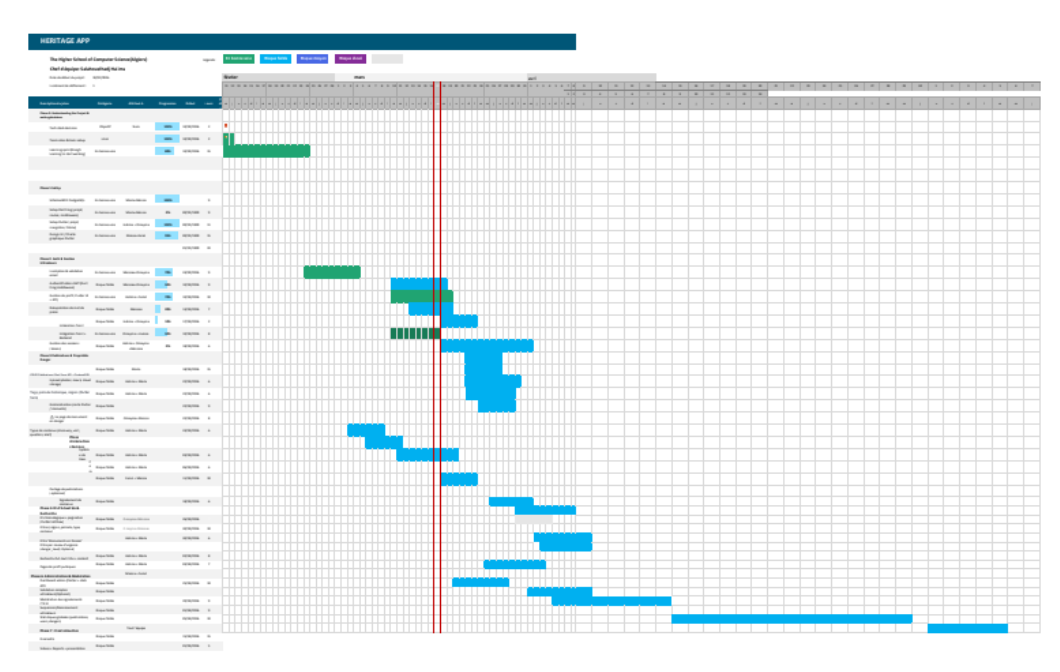
\includegraphics[width=1\textwidth, trim=0 0 0 0]{images/planning1.png}
\end{center}

\subsection{Project Management Tools}
To enhance our organization and maximize efficiency, we implemented a comprehensive set of project management tools, which can be categorized into three main areas:

\subsubsection{Communication and Collaboration}
\begin{minipage}{0.7\textwidth}
\textbf{Discord}
is an online communication platform originally designed for gamers but now widely adopted by various communities and professional teams. It enables real-time text and voice communication, along with seamless file and media sharing.

We leveraged Discord by creating a dedicated server where all project-related information was centralized. This space served as a hub for sharing relevant resources, conducting discussions about ongoing tasks, and organizing meetings, work sessions, and collaborative exchanges.
By utilizing structured channels and customized permission settings, we ensured clear, well-organized communication, allowing information to flow efficiently and reach the right team members at the right time.
\end{minipage}
\begin{minipage}{0.3\textwidth}
\centering
    
\includegraphics[width=0.7\linewidth]{images/DiscordLogo.png}
    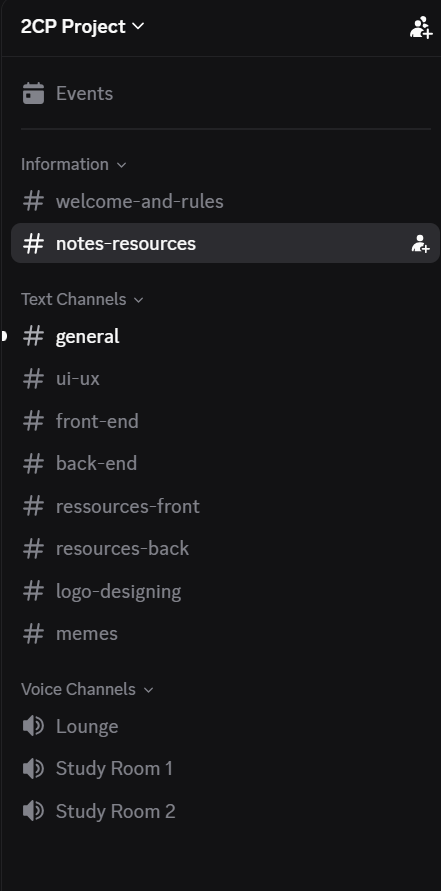
\includegraphics[width=0.7\linewidth]{images/discordGroup.png}
\end{minipage}

\begin{minipage}{0.7\textwidth}
\textbf{Google Meet}
enabled seamless and efficient collaboration among team members during project meetings. It facilitated productive work sessions and ensured clear, transparent communication throughout the project. Its intuitive interface and smooth integration with other digital tools significantly improved coordination and enhanced overall team performance.
\end{minipage}
\begin{minipage}{0.3\textwidth}
\centering
    
\includegraphics[width=0.7\linewidth]{images/GoogleMeet.png}
\end{minipage}

\begin{minipage}{0.7\textwidth}
\textbf{Gmail}
played a central role in facilitating formal communication within the project team. It was used to exchange important documents, share updates, and ensure reliable information flow between members. Its organization features, such as labels, filters, and threaded conversations, helped maintain clarity and structure in all project-related correspondence, improving efficiency and traceability.
\end{minipage}
\begin{minipage}{0.3\textwidth}
\centering
    
\includegraphics[width=0.7\linewidth]{images/GmailLogo.png}
\end{minipage}

\begin{minipage}{0.7\textwidth}
\textbf{Google Drive}
 was used as a centralized storage system for all project files and resources. It allowed us to store, organize, and share documents, assets, and references securely. This ensured that every team member had access to the latest versions of files at any time, improving consistency and avoiding duplication or loss of data.
\end{minipage}
\begin{minipage}{0.3\textwidth}
\centering
    
\includegraphics[width=0.7\linewidth]{images/GoogleDriveLogo.png}
\end{minipage}

\begin{minipage}{0.7\textwidth}
\textbf{Google Docs}
 was essential for collaborative documentation. It allowed multiple team members to write, edit, and comment on the project report simultaneously. This real-time collaboration improved efficiency and ensured consistency in the final documentation.
\end{minipage}
\begin{minipage}{0.3\textwidth}
\centering
    
\includegraphics[width=0.7\linewidth]{images/GoogleDocsLogo.png}
\end{minipage}

\begin{minipage}{0.7\textwidth}
\textbf{Microsoft Excel}
 was used as an effective tool for project planning and task management through the creation of a Gantt chart. It allowed us to organize tasks clearly, define their start and end dates, and visualize the overall project timeline. This helped each team member understand their responsibilities and deadlines.
The Gantt chart also enabled us to track the progress of tasks throughout the project and quickly identify any delays or overlaps. Additionally, Excel provided the flexibility to update the schedule when needed, ensuring that our planning remained accurate and up to date. Overall, it contributed to better time management, coordination, and organization within the team.
\end{minipage}
\begin{minipage}{0.3\textwidth}
\centering
    
\includegraphics[width=0.7\linewidth]{images/Excel Logo.png}
\end{minipage}

\begin{minipage}{0.7\textwidth}
\textbf{GitHub}
 served as the central platform for version control and collaborative development throughout the project. It allowed us to manage the codebase in an organized way using branches, enabling each team member to work on separate features independently without interfering with others’ work. Regular commits were used to document progress and track changes, which made it easy to review modifications and revert to previous versions when necessary. GitHub also helped us maintain a clean workflow and efficiently merge contributions from different members.
\end{minipage}
\begin{minipage}{0.3\textwidth}
\centering
    
\includegraphics[width=0.7\linewidth]{images/GitHubLogo.png}
\end{minipage}

\begin{minipage}{0.7\textwidth}
\textbf{Figma}
 played a crucial role in the design phase of the project. It enabled collaborative UI/UX design in real time, allowing the team to create, modify, and refine interface prototypes together. This helped us visualize the application structure early and ensure design consistency across all screens before development.
\end{minipage}
\begin{minipage}{0.3\textwidth}
\centering
    
\includegraphics[width=0.7\linewidth]{images/FigmaLogo.png}
\end{minipage}

\begin{minipage}{0.7\textwidth}
\textbf{Canva}
 was used to create visual content such as presentations and design elements. It helped us produce clean, attractive, and professional visuals, improving the overall presentation quality of the project.
\end{minipage}
\begin{minipage}{0.3\textwidth}
\centering
    
\includegraphics[width=0.7\linewidth]{images/CanvaLogo.png}
\end{minipage}

\begin{minipage}{0.7\textwidth}
\textbf{Overleaf}
  was the main platform used for writing and formatting the project report. It provided a collaborative LaTeX environment that allowed all team members to work on the same document simultaneously in real time. This made it easier to structure the report professionally, manage sections efficiently, and ensure consistency in formatting throughout the document.
In addition, Overleaf simplified the process of handling references, equations, and layout organization, which are often complex in traditional word processors. Its cloud-based nature allowed us to access and edit the report from anywhere without the need for manual file sharing. Overall, Overleaf played a crucial role in producing a well-structured, clean, and professional final report.
\end{minipage}
\begin{minipage}{0.3\textwidth}
\centering
    
\includegraphics[width=0.7\linewidth]{images/LataxLogo.png}
\end{minipage}

\vspace{1cm}

\textbf{Conclusion}

Overall, the combination of these tools significantly enhanced our teamwork and productivity throughout the project. They allowed us to maintain clear communication, organize tasks efficiently, and collaborate seamlessly across different stages of development and design. By integrating platforms such as GitHub, Discord, Google Meet, and others, we were able to ensure a structured workflow, reduce misunderstandings, and improve coordination between all team members. This effective use of collaborative tools played a key role in the successful completion of our project.
\subsection{Risk Management}
Risk management is an essential component of any project, aimed at identifying, evaluating, and mitigating factors that may hinder the achievement of objectives. In this section, we detail the challenges encountered during the development of the Rawasii project and the strategies adopted to overcome them effectively.
\subsubsection{Time Management}
One of the primary difficulties faced at the outset of the project was time management. The team initially struggled to distribute tasks efficiently and maintain a consistent pace of development. However, this issue was progressively resolved through improved planning, clearer task allocation among team members, and the adoption of a more structured workflow that allowed the project to stay on track despite early setbacks.
\subsubsection{Front-End and Back-End Integration}
Another significant challenge arose during the integration phase between the front-end and back-end components of the application. Connecting the different parts of the system revealed compatibility issues and communication gaps between the two sides. These were addressed through better coordination between team members and more rigorous testing during the integration phase, ensuring the overall system functioned cohesively.
\subsubsection{Hardware Limitations}
On the technical side, one team member experienced performance issues with Flutter development due to insufficient RAM on her laptop, which disrupted her ability to run the application locally. This was resolved by turning to online compilation tools, enabling her to continue contributing to the project without interruption and without compromising the overall development timeline.

Overall, these challenges served as valuable learning experiences. They strengthened the team's problem-solving capabilities, fostered better communication, and reinforced collaboration — all of which contributed positively to the quality and resilience of the final product.

\newpage

\section{Conception}
\subsection{Introduction}
The design phase represents the core foundation of any project and a decisive step toward its success. It plays a crucial role in clarifying project objectives, defining system functionalities, and evaluating different possible solutions to address the identified problem, all based on a thorough analysis of the specifications document. During this phase, key architectural and functional decisions are made to guide the development process effectively.

The primary goal of this stage is to ensure that the final product accurately satisfies user requirements, remains technically feasible within the available resources, and complies with time constraints. A well-executed design phase significantly reduces risks during implementation and improves the overall quality, coherence, and efficiency of the final system.
\subsection{User Flow}
In project design, the user flow plays a fundamental role in creating an optimal user experience and ensuring the overall success of the system. Also known as the user journey, it represents the sequence of steps and actions a user follows to achieve a specific goal within an application. It is typically illustrated as a diagram that maps the path taken by the user and highlights their interactions with the system at each stage of the process.
\subsubsection{Authentication and Access}
This is the first step when the user interacts with the application.
The user can either sign up or log in.
During sign up, the user provides basic information such as name, email, and password.
After successful authentication, the user is redirected to the home page.
\subsubsection{Core User Experience}
This section represents the main functionalities of the application that users interact with daily.
\begin{itemize}
    \item Home Feed
    
Displays posts related to tourist landmarks in Algeria.
Users can view shared content from other users.
    \item Popular Section

    Shows the most viewed and most engaging posts.
Helps users discover trending content.
    \item Search

    Users can search for:
    
Posts

Tourist landmarks

This allows quick access to specific content.
    \item  Create Post

Users can create posts about tourist landmarks.

Posts may include text and images.

Published posts appear in the main feed.
     \item Comments
\end{itemize}
\subsubsection{Community and Safety Features}
This section focuses on collaboration, awareness, and platform safety.
\begin{itemize}
    \item Endangered Landmarks
    
Displays landmarks that are at risk or endangered.

Includes awareness information about their importance.

Users can organize campaigns to support and protect these landmarks.
    \item  Groups
    
Users can create or join groups.

Groups allow sharing posts and discussions about landmarks.

Encourages community interaction.
    \item Report System
    
Users can report inappropriate posts or content.

Reports are sent to the administration for review.
     \item Administration
     
The admin manages the platform content and user activity.

Reviews reported posts and comments.

Takes actions such as removal of content or warnings.

Oversees campaigns in the endangered landmarks section.

Ensures safety, quality, and proper use of the application.
\end{itemize}
\subsection{Database Schema}
\begin{center}

    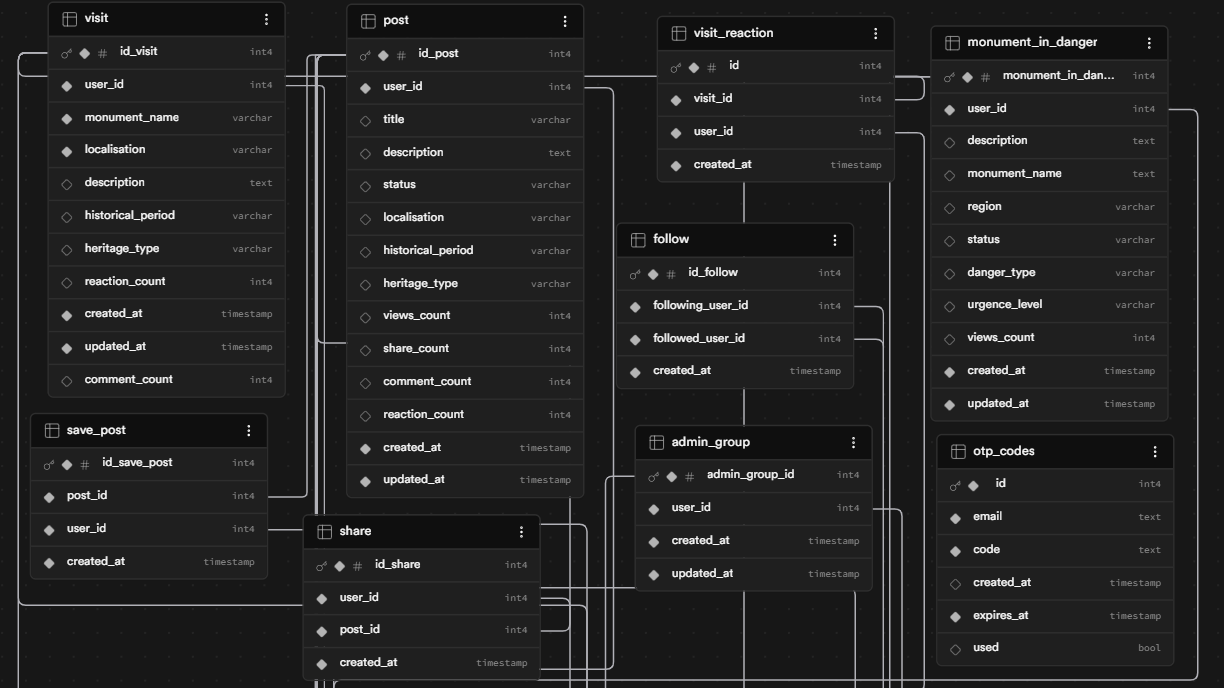
\includegraphics[width=0.7\linewidth]{images/db1.png}

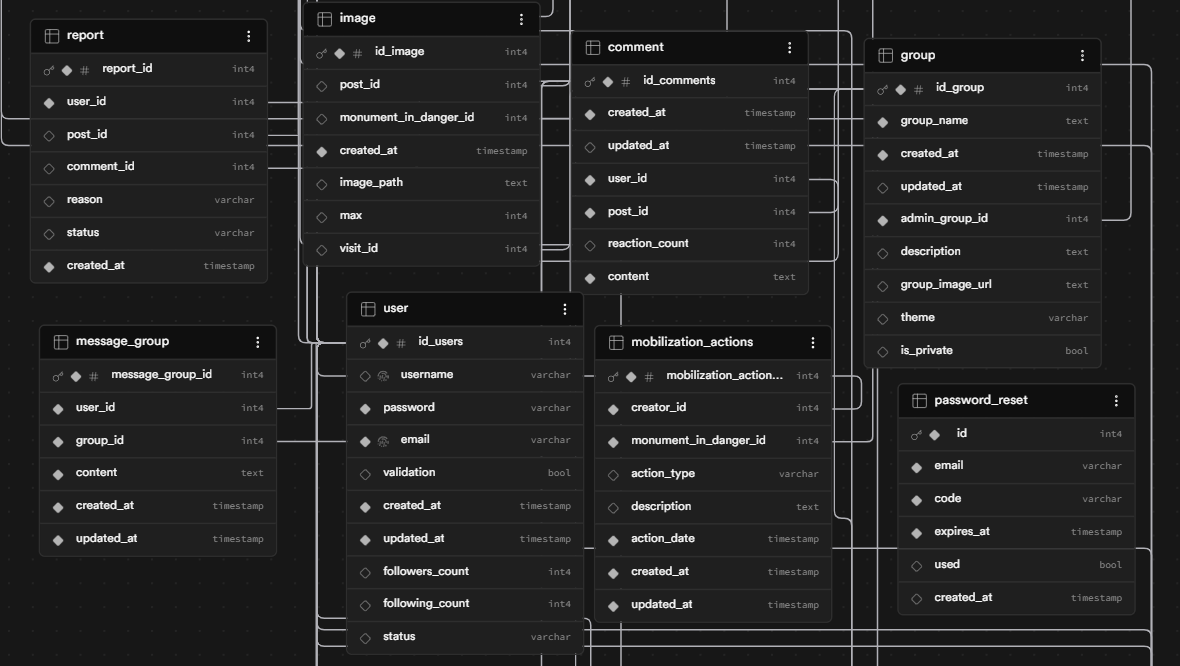
\includegraphics[width=0.7\linewidth]{images/db2.png}

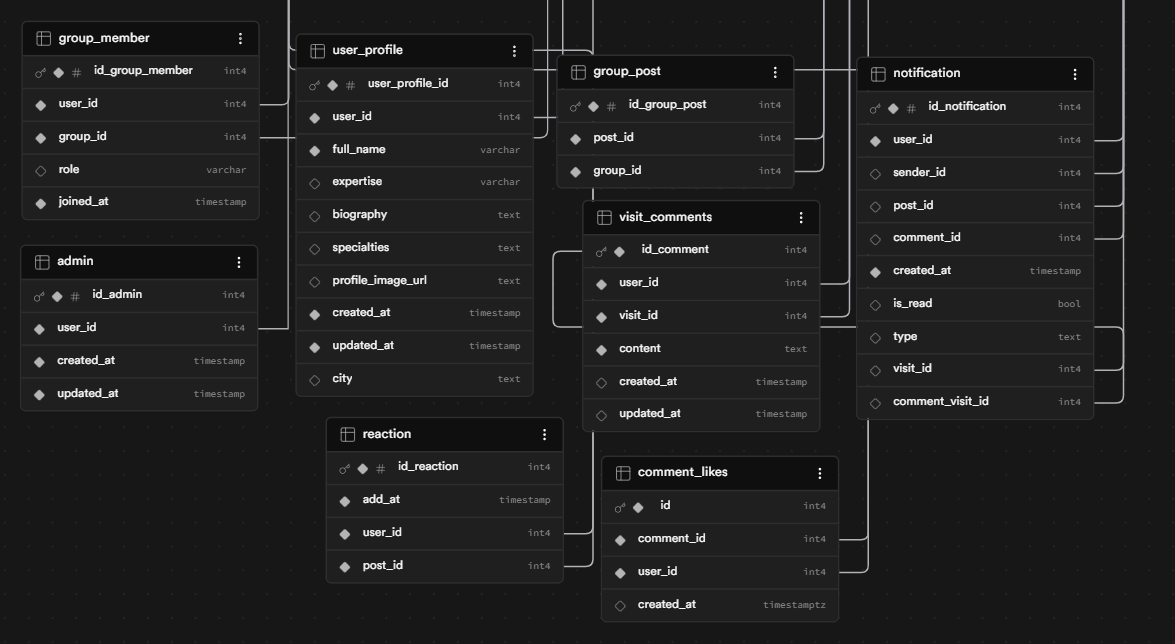
\includegraphics[width=0.7\linewidth]{images/db3.png}

\end{center}



\subsection{Modular Breakdown}
The modular breakdown of a software system is a design approach that consists of dividing the system into autonomous and interconnected modules, each responsible for a specific functionality. This allows for better organization, easier maintenance, and a greater ability to evolve the software over time.
To structure Rawasii in a modular way, we began by carefully analyzing the project requirements and defining all functionalities during the design phase. We then opted for a grouping approach, organizing features first into systems, then into broader super-systems.
\subsubsection{Authentication Module}
The Authentication module represents the entry point of the Rawasii application, ensuring secure and controlled access to the platform. It is composed of three core functions:

The Connection function receives two inputs — the user's email and password — and grants access to their account upon successful validation. In case of invalid credentials, it returns an error message to inform the user.
The Disconnection function allows any logged-in user to safely log out of the application, terminating their active session.

The Create an Account function handles the registration of new users by collecting four pieces of information: email, password, username, and user type. This last field distinguishes between different user roles on the platform. Like the connection function, it returns an error message if the registration process fails.

Together, these three functions form a complete and secure authentication flow that controls who can access Rawasii and in what capacity.

\vspace{0.5cm}

\begin{center}

    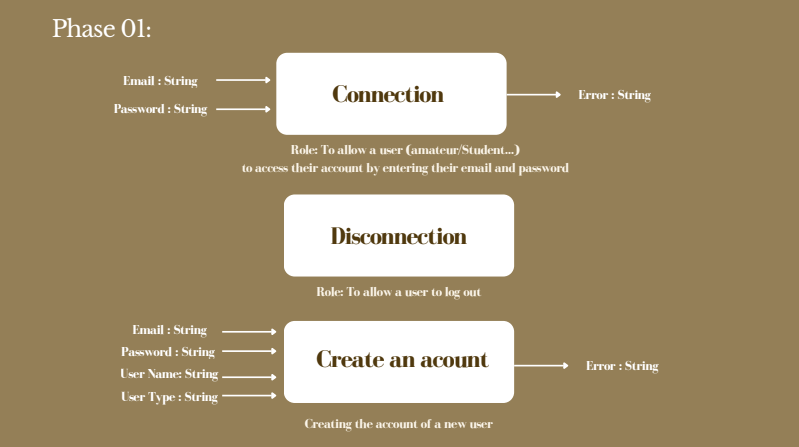
\includegraphics[width=0.9\textwidth]{images/phase1.png}
    
\end{center}

\subsubsection{ Publication Module}
The Publication module enables users to share and manage heritage content on the platform. It consists of two main functions:

The Add a New Post function allows users to create and publish a heritage post by providing several inputs: multimedia content, filter elements through checkboxes for categorization, an optional location, and a boolean field indicating whether the monument is in danger. This last field serves an important awareness purpose within the platform. The function returns an error message if the submission fails.

The Delete/Edit a Post function gives users control over their published content, allowing them to modify an existing post or remove it entirely, as well as update the status of the monument featured in the post. It also returns an error message in case of failure.

\vspace{0.5cm}

\begin{center}
    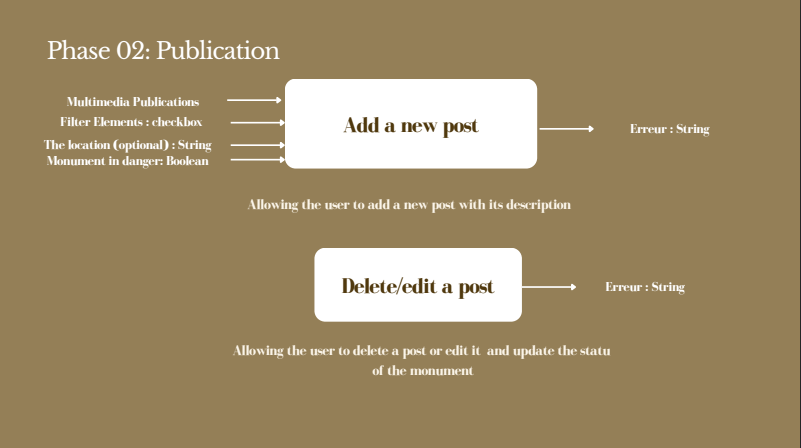
\includegraphics[width=0.9\textwidth]{images/phase2.png}
\end{center}

\subsubsection{Social Interaction Module}

The Social Interaction module covers all the ways users can engage with heritage content on the platform. It is composed of four functions:
The Add a Reaction function allows users to express their feelings toward a post by selecting a reaction through a checkbox, enabling quick and expressive engagement.

The Add a Comment/Reply function lets users leave a comment or reply to an existing one, accepting a text input between 1 and 500 characters, ensuring meaningful yet concise interactions.

The Share a Publication function enables users to spread heritage content beyond the platform by sharing posts through various external channels.
The Report a Publication function allows users to flag inappropriate or incorrect content by submitting a report reason as a text input, contributing to the quality and integrity of the platform.

\vspace{0.5cm}

\begin{center}
    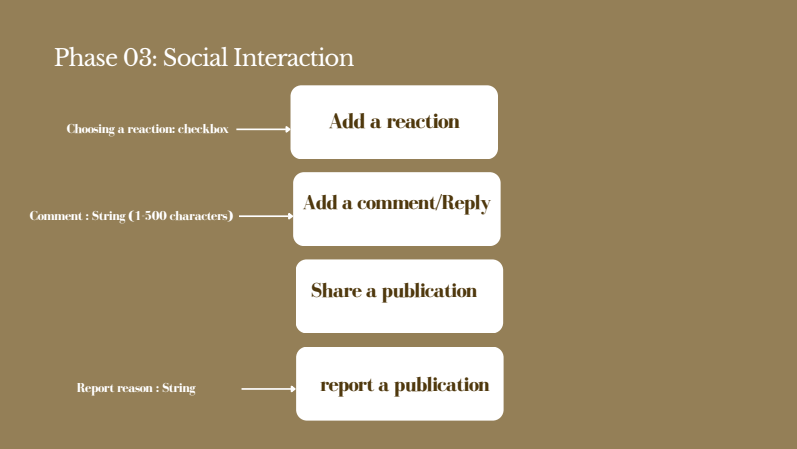
\includegraphics[width=0.9\textwidth]{images/phase3.png}
\end{center}


\subsubsection{Search and News Feed Module}

The Search and News Feed module enables users to discover content and navigate the platform efficiently. It revolves around one core function:

The Search function accepts two inputs: a keyword as a text string, and filtering options through checkboxes to narrow down the results. This allows users to search for both profiles and heritage places, and to refine their results to display only the specific content they are looking for.

\vspace{0.5cm}

\begin{center}
    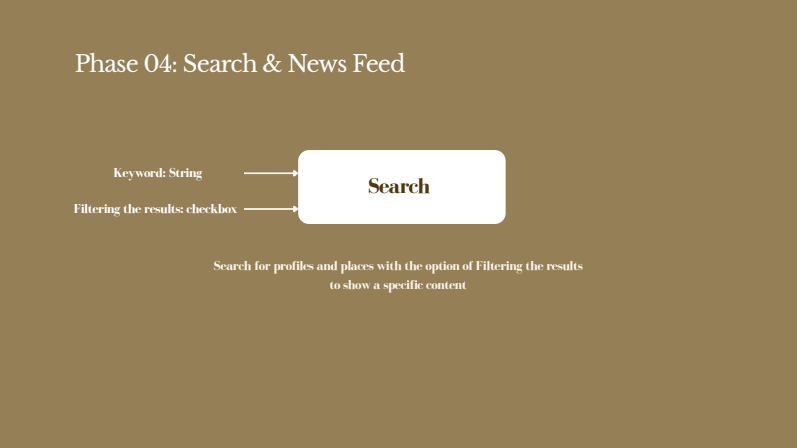
\includegraphics[width=0.9\textwidth]{images/phase4.png}
\end{center}


\subsubsection{Administration and Moderation Module}

The Administration and Moderation module grants platform administrators the tools needed to maintain a safe and trustworthy environment. It is composed of three functions:

The Moderation of Reports function allows admins to review user-submitted reports by examining the report reason provided as a text input, and taking appropriate action on flagged content.

The User Suspension/Banning function gives administrators the ability to restrict access for users who violate platform rules, either temporarily through suspension or permanently through banning.

The Overall Statistics function provides admins with a comprehensive overview of the platform's activity, covering key metrics related to publications, users, and at-risk monuments, enabling informed decision-making and platform monitoring.

\vspace{0.5cm}

\begin{center}
    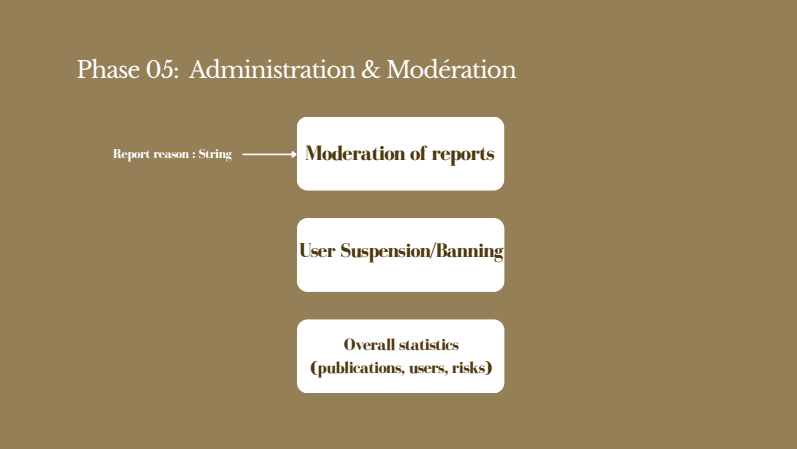
\includegraphics[width=0.9\textwidth]{images/phase5.png}
\end{center}


\subsubsection{System Outputs}

The Rawasii system produces the following outputs:

Member Profiles — personalized user pages displaying identity, interests, and published content. Filtered News Feed — a paginated and filterable stream of heritage publications tailored to the user's preferences.

Heritage Map — an interactive map displaying geolocated monuments, with endangered sites clearly marked. At-Risk Publications — posts flagged by the danger indicator, filtered by urgency level to prioritize critical heritage alerts. Search Results — content filtered by historical period, region, type, and danger status to deliver precise and relevant results.

Notifications — real-time alerts covering replies, reactions, and annotation validations. Admin Dashboard — a centralized panel providing global statistics, reported content, and moderation tools for platform administrators.
\subsection{Graphic charter and visual identity}
\subsubsection{ Name and Logo}

The name "Rawasii" was chosen because it reflects stability, authenticity, and deep roots, values that strongly relate to Algerian architectural heritage.

The word is inspired by the writings of Ibn Khaldun in Al-Muqaddimah, symbolizing firmness and cultural continuity across generations.

Our project aims to preserve and strengthen the connection between Algerians and their architectural heritage by presenting traditional monuments, designs, and historical identities in a modern digital form.

The logo was designed to visually represent Algerian architectural identity through elements inspired by traditional structures and cultural symbols, combining heritage with modern technology.

\begin{center}
    
\includegraphics[width=0.7\linewidth]{images/logo-1-primary.png}
\end{center}
    

\subsubsection{Typography (Font)}
\begin{minipage}{0.55\textwidth}
   The Tajawal font was selected for this project because it is a modern typeface characterized by clarity, simplicity, and excellent readability across different screen sizes. It is also a versatile font that supports both Arabic and Latin scripts, making it suitable for an application intended for users from diverse regions around the world. This font contributes to enhancing the visual user experience by providing a clean and well-structured interface that reflects the modern identity of the application.
\end{minipage}
\begin{minipage}{0.45\textwidth}
\centering
    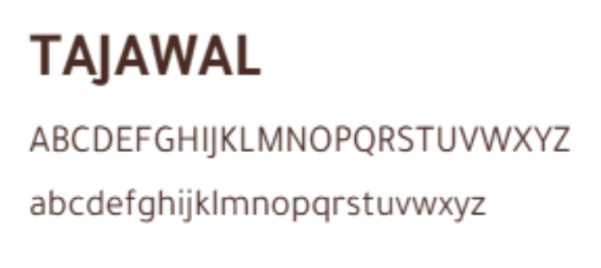
\includegraphics[width=0.9\linewidth]{images/font.png}
\end{minipage}
\subsubsection{Color Palette}
Colors play a fundamental role in this project, as each shade directly influences the user’s emotions and perception. This has led to the selection of a coherent palette inspired by Algerian heritage, where each color conveys a specific meaning and contributes to the visual identity of the platform. 

\begin{center}
    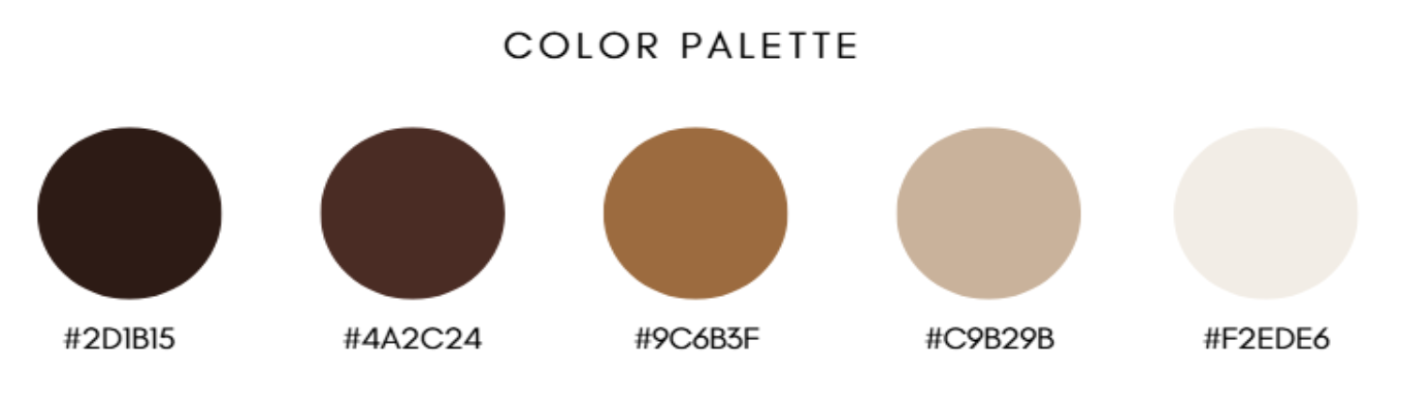
\includegraphics[width=0.8\linewidth]{images/colors.png}
\end{center}


\#2D1B15 : It helps organize the interface and reinforces information hierarchy. 

\#4A2C24 : It is used for titles and important elements to ensure strong readability. 

\#9C6B3F : This color reflects traditional elements such as pottery, wood, and desert landscapes. 

\#C9B29B : It introduces a soft traditional touch inspired by natural and cultural Algerian tones. 

\#F2EDE6 : It is used as the main background color to ensure comfortable reading and highlight content without distraction. 
\subsection{UI UX Design}
\subsubsection{Introduction}
The UI/UX design phase focused on creating an interface that is visually attractive, easy to use, and provides a smooth user experience. Special attention was given to the organization of elements, navigation simplicity, and the overall appearance of the application in order to make the interaction intuitive and comfortable for users.

\begin{center}

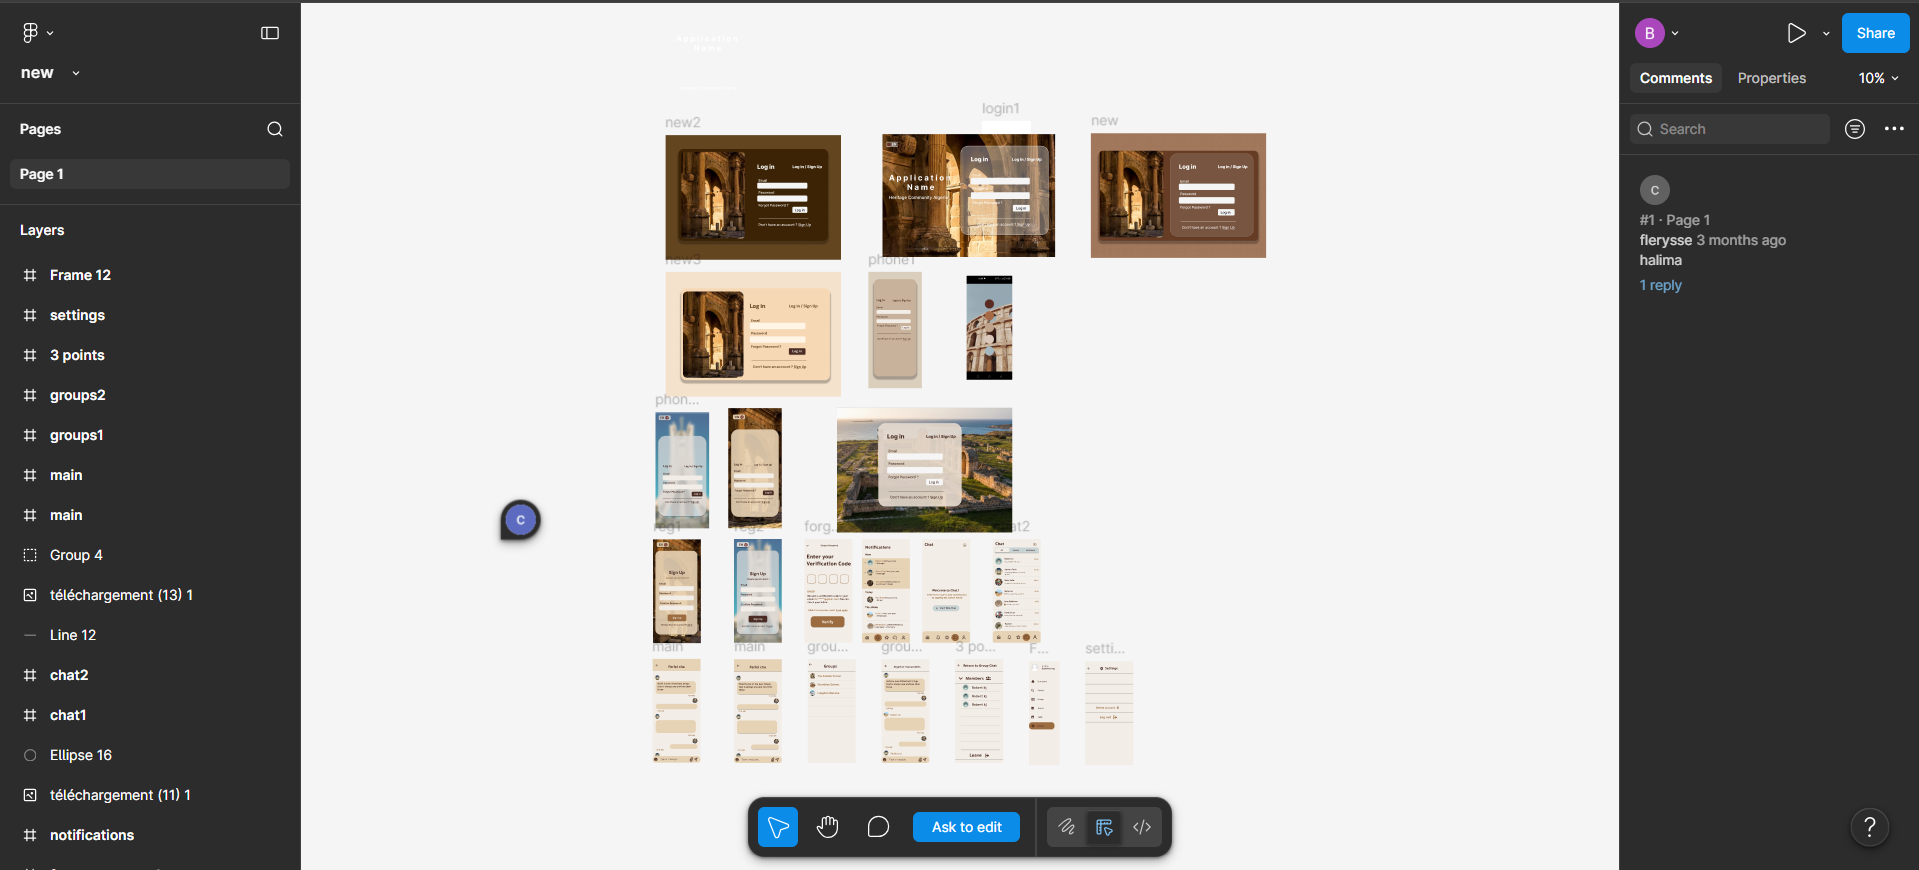
\includegraphics[width=1\linewidth]{images/ui1.png}

\vspace{0.5cm}

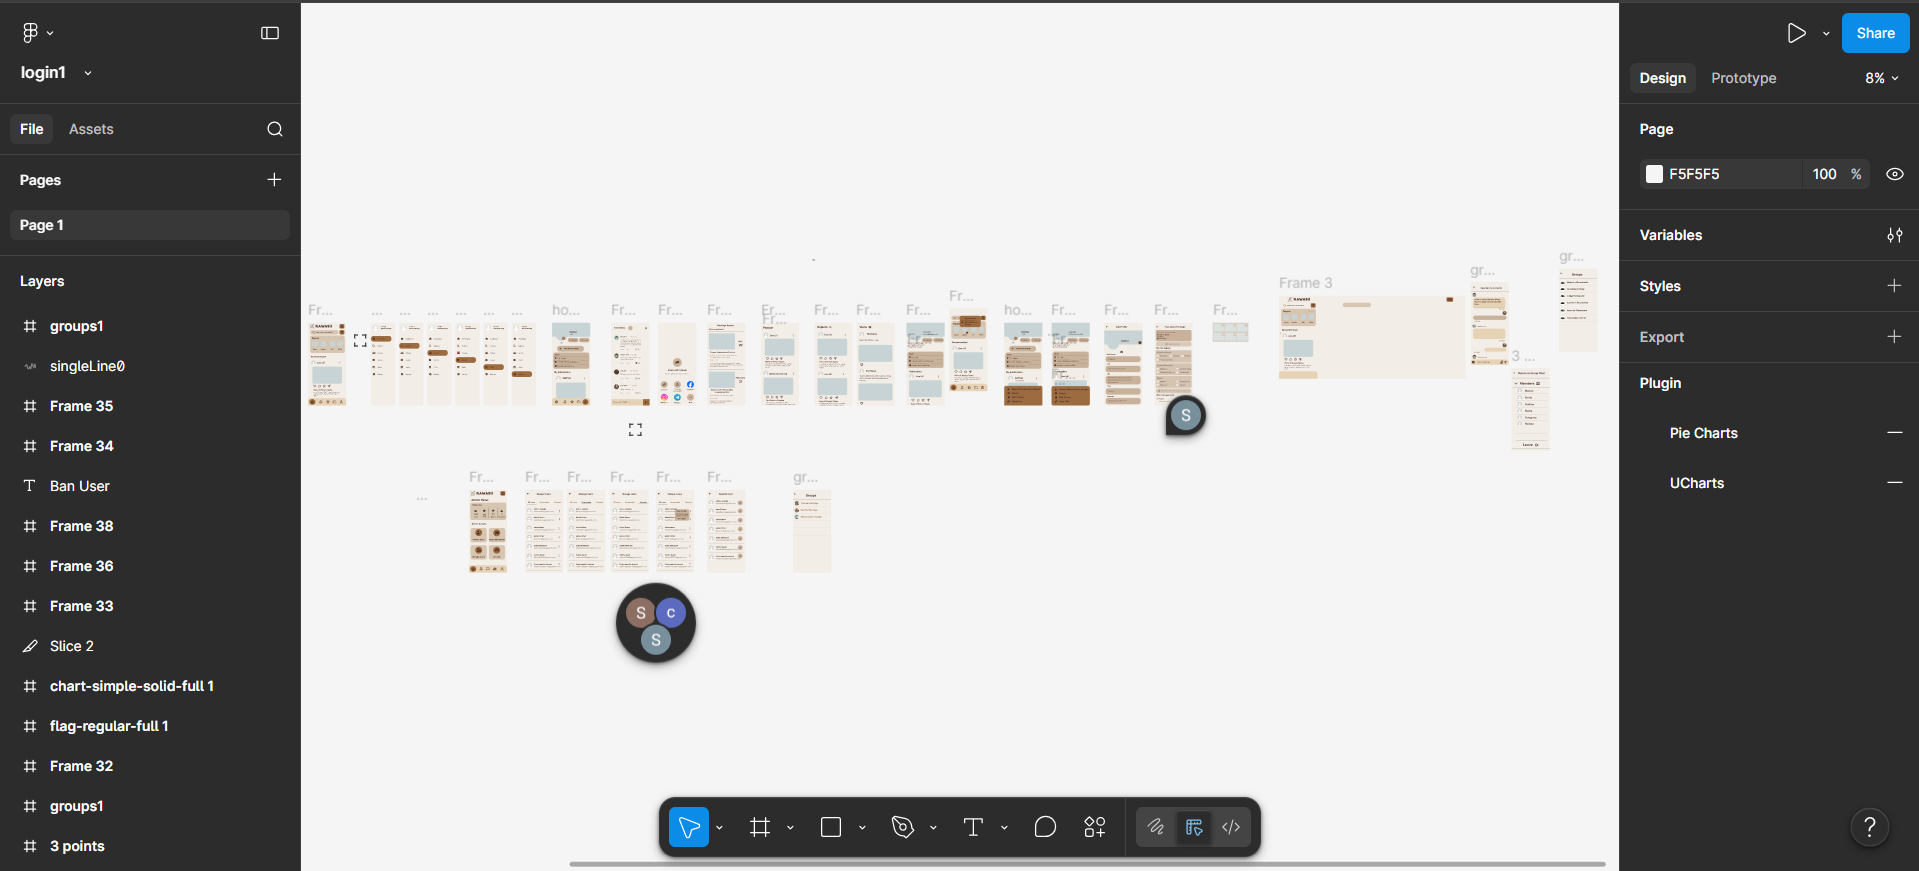
\includegraphics[width=1\linewidth]{images/ui2.png}
    
\end{center}


\subsubsection{Designing the User Interface}
The user interface was designed using Figma, which allowed the creation of organized and interactive layouts before starting the development phase. Through Figma, different screens of the application were designed while respecting consistency in colors, typography, spacing, and component placement.

The design process focused on creating a modern and clean interface that reflects the purpose of the application while maintaining simplicity and clarity.

\subsubsection{User Experience Considerations}
During the UI/UX phase, several user experience principles were taken into consideration to improve usability and accessibility. Navigation between screens was designed to be simple and intuitive, allowing users to interact with the application efficiently without confusion.

Attention was also given to the arrangement of buttons, menus, and content sections in order to provide a smooth and comfortable experience for different types of users.
\subsubsection{Prototyping and Visualization}
Figma was also used to create prototypes and visualize how users would interact with the application before implementation. This helped identify possible design improvements early in the project and reduced potential issues during development.
\subsubsection{Advantages of Using Figma}
Using Figma provided flexibility and efficiency during the design process. It simplified collaboration, accelerated interface creation, and allowed easy modification of components and layouts throughout the project development cycle.

\newpage

\section{Implementation}
\subsection{Introduction}
Following a successful design phase, the project progresses to the implementation stage of the software. This phase involves developing the various functionalities independently on both the front-end and back-end levels, and then integrating them to produce a coherent and fully functional final product.

Special emphasis is placed on testing throughout this stage to refine, optimize, and enhance the system. This process ensures that the software meets quality standards, performs efficiently, and delivers a stable and reliable user experience.
\subsection{Tools and Technologies Used}
\begin{minipage}{0.8\textwidth}
\textbf{VS Code}
 was used as the main development environment for writing and managing the project code. It provided a lightweight interface with useful extensions that improved productivity and simplified debugging.
\end{minipage}
\begin{minipage}{0.2\textwidth}
\centering
    
\includegraphics[width=0.7\linewidth]{images/VScodeLogo.png}
\end{minipage}
\begin{minipage}{0.8\textwidth}
\textbf{Flutter}
 was used as the frontend framework to build the user interface of the application. It enabled us to create a responsive and consistent UI across different devices using a single codebase.
\end{minipage}
\begin{minipage}{0.2\textwidth}
\centering
    
\includegraphics[width=0.7\linewidth]{images/Flutter Vector Logo.jpg}
\end{minipage}
\begin{minipage}{0.8\textwidth}
\textbf{Dart}
  was the primary programming language used in the project. It was mainly used with Flutter and Dart Frog, ensuring efficient and structured development.
\end{minipage}
\begin{minipage}{0.2\textwidth}
\centering
    
\includegraphics[width=0.7\linewidth]{images/dartLogo.png}
\end{minipage}
\begin{minipage}{0.8\textwidth}
\textbf{ Dart Frog}
was used to develop the backend of the application. It allowed us to build APIs and handle server-side logic in a simple and organized way.
\end{minipage}
\begin{minipage}{0.2\textwidth}
\centering
    
\includegraphics[width=0.7\linewidth]{images/dart frog.png}
\end{minipage}
\begin{minipage}{0.8\textwidth}
\textbf{Git}
  was used as a version control system to track changes and manage collaboration between team members. It helped maintain a clean and organized development workflow.
\end{minipage}
\begin{minipage}{0.2\textwidth}
\centering
    
\includegraphics[width=0.7\linewidth]{images/Git.jpg}
\end{minipage}
\begin{minipage}{0.8\textwidth}
\textbf{Supabase}
  was used as the backend-as-a-service platform, providing a PostgreSQL database along with features such as authentication and real-time data handling, which simplified backend development and data management.
\end{minipage}
\begin{minipage}{0.2\textwidth}
\centering
    
\includegraphics[width=0.7\linewidth]{images/supabaseLogo.png}
\end{minipage}
\begin{minipage}{0.8\textwidth}
\textbf{pgAdmin 4}
 was used as a database management tool to interact directly with the PostgreSQL database. It allowed us to create tables, manage data, execute SQL queries, and monitor the database structure in an efficient and user-friendly way.
\end{minipage}
\begin{minipage}{0.2\textwidth}
\centering
    
\includegraphics[width=0.7\linewidth]{images/PostgresLogo.jpg}
\end{minipage}
\begin{minipage}{0.8\textwidth}
\textbf{Docker}
  was used to containerize the application and ensure a consistent development and deployment environment. It allowed us to package the backend and its dependencies into isolated containers, making the application easier to run across different machines without configuration issues.
  
Additionally, Docker simplified the setup process and improved portability, especially when working on different devices. It also helped maintain consistency between development environments and reduced potential compatibility problems.
\end{minipage}
\begin{minipage}{0.2\textwidth}
\centering
    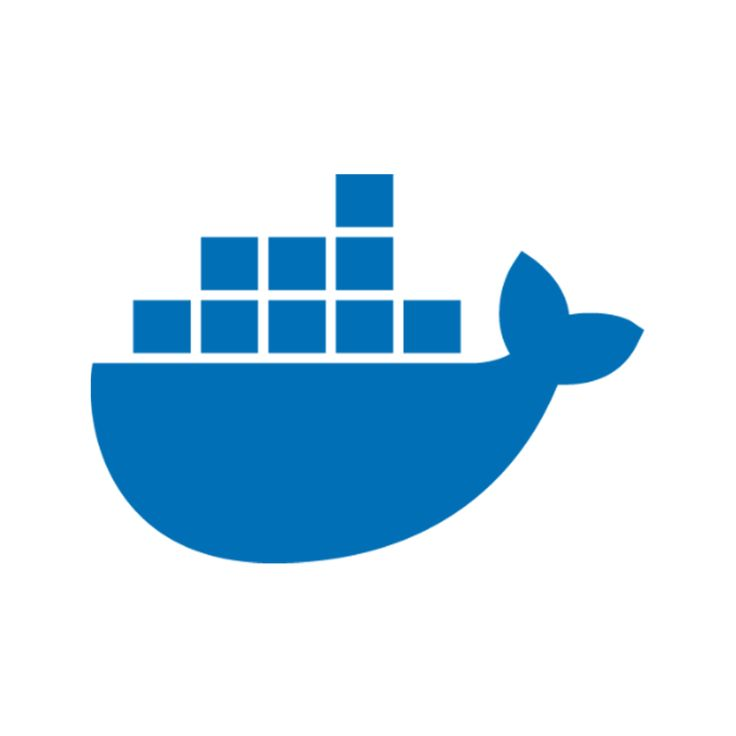
\includegraphics[width=0.7\linewidth]{images/Docker Logo.png}
\end{minipage}
\subsection{Database}
\subsubsection{Introduction}
The database is a fundamental component of the application, used to store and organize data in a way that ensures easy access, integrity, and efficient performance during usage.
\subsubsection{Local Database Management}
At the beginning of the project, pgAdmin 4 was used as a local PostgreSQL database management tool. It helped in creating tables, testing relationships between data, and executing various SQL commands during the early development phase, which provided a better understanding of the database structure before moving to the final environment.
\subsubsection{Cloud Database Integration}
Later, the project was migrated to Supabase, a cloud-based platform built on PostgreSQL that provides an integrated environment for managing and connecting the database directly with the application. This transition allowed remote access to the database and improved development and deployment efficiency.
\subsubsection{Database Structure}
The data was organized into relational tables to reduce redundancy and ensure data integrity. Relationships between tables were designed logically to allow efficient and fast data management.
\subsubsection{Advantages of the Chosen Solution}
Using Supabase with PostgreSQL improved the application’s performance by providing automatic APIs, authentication support, easier scalability, and a stable and secure data environment.

\vspace{0.5cm}
\begin{center}

    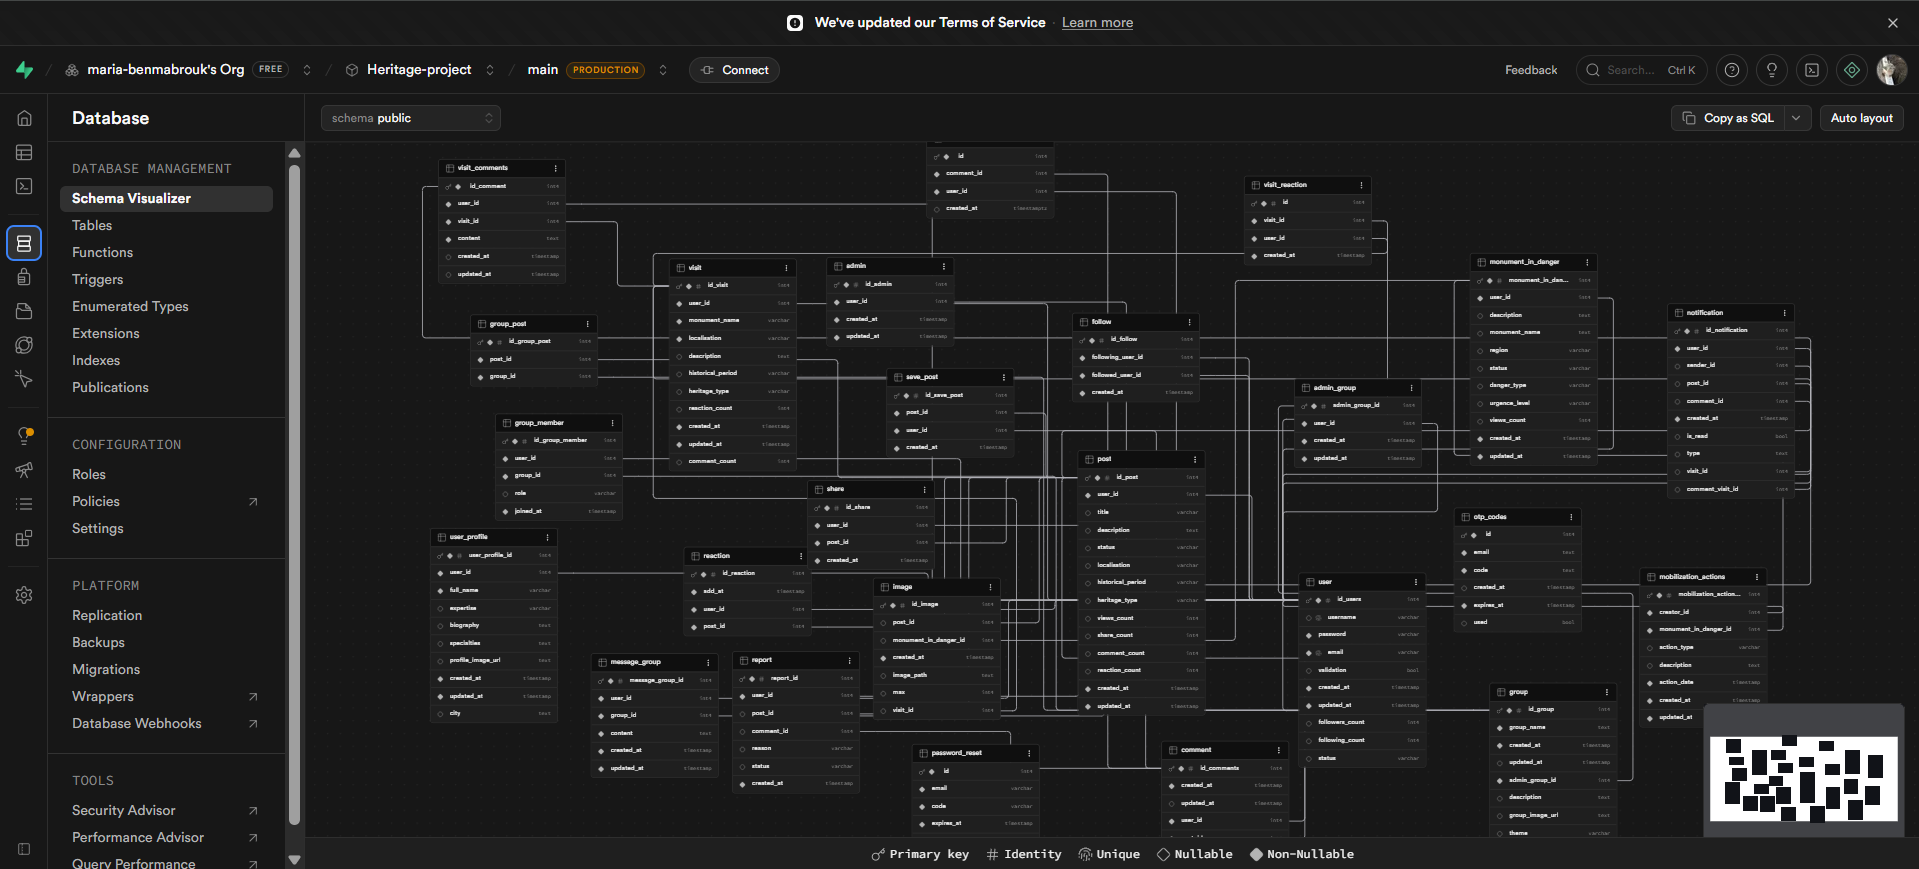
\includegraphics[width=1\textwidth]{images/supabase1.png}

\vspace{0.5cm}

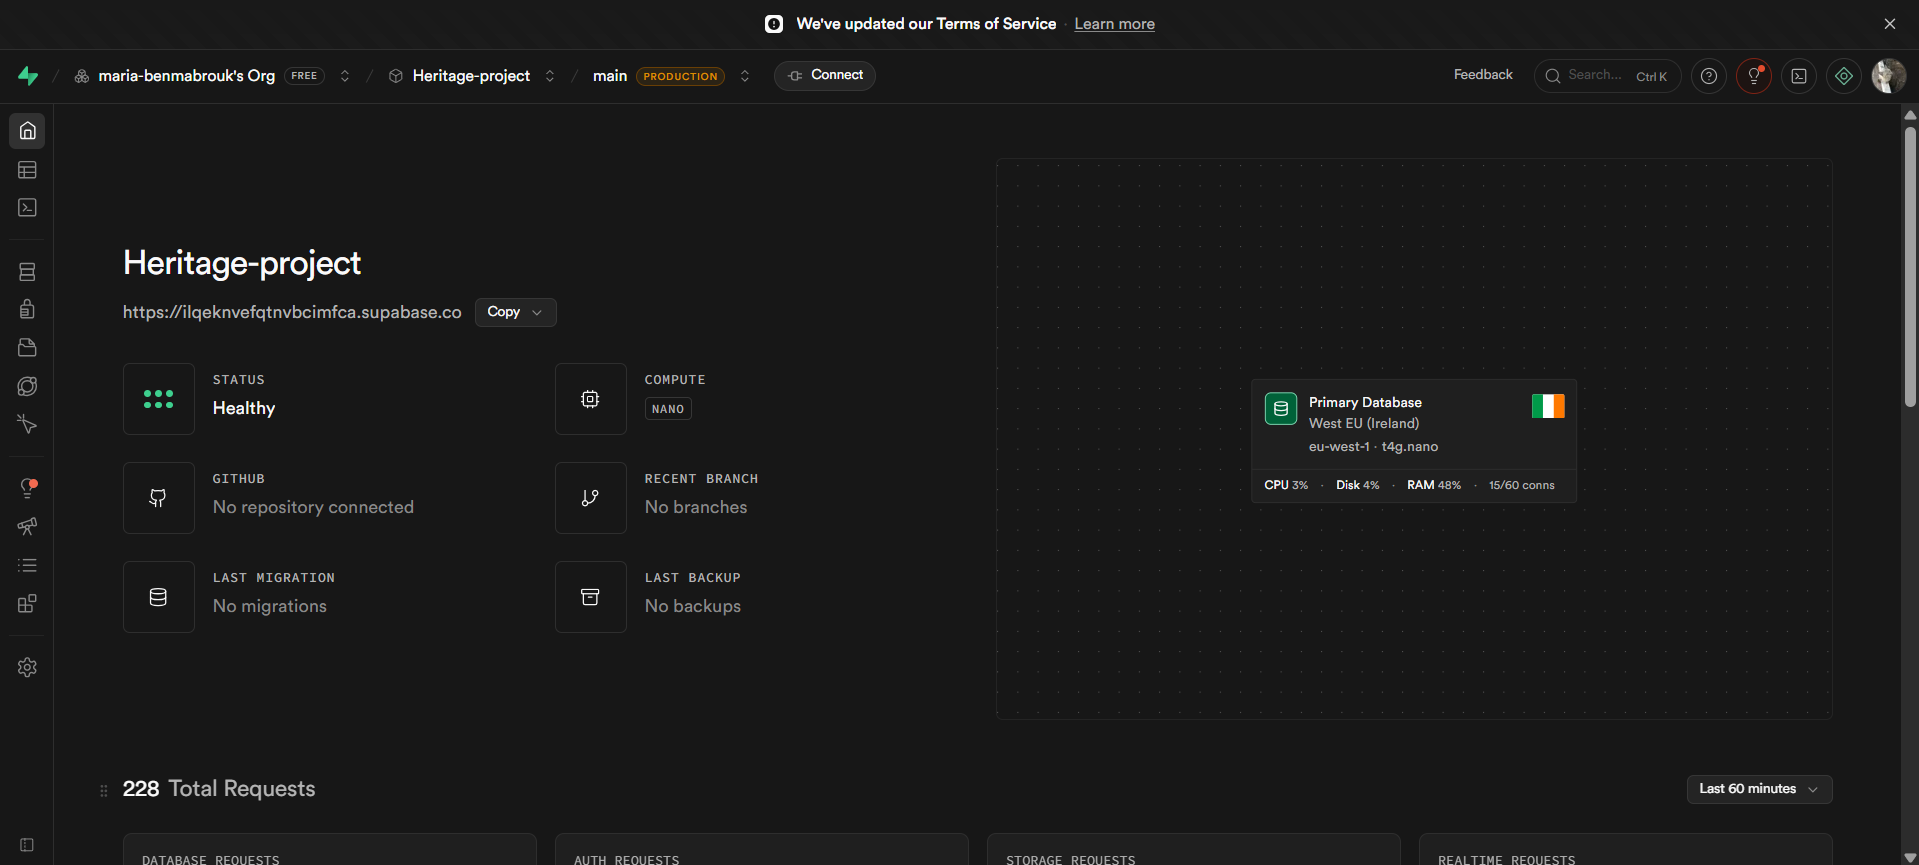
\includegraphics[width=1\textwidth]{images/supabase2.png}

\end{center}

\subsection{Front-end}
\subsubsection{Introduction}
The front-end part of a web application represents the interface through which users directly interact with the system. It includes all visible and interactive elements of the application, as well as the functionalities associated with them. Front-end development plays an essential role in creating an intuitive, responsive, and engaging user experience.

In the development of the front-end part of our project, we chose to use Flutter and Dart. These modern technologies enabled us to build a dynamic and responsive application with an attractive and user-friendly interface.

Our project is a social networking platform dedicated to Algerian architectural heritage. The application allows users to share publications, interact with other members, participate in thematic discussions, and explore heritage-related content through a collaborative environment.

For the realization of this important part of the project, we relied on Flutter’s flexible UI system and Dart’s programming capabilities to create modern interfaces and ensure smooth interaction between users and the application.

\subsubsection{Frontend Implementation According to the Design}

\textbf{Translation of the Design into Flutter Widgets}

We started by transforming the interface mockups into Flutter widgets. Each visual element was divided into reusable and modular components while paying particular attention to responsiveness and interface consistency.

\textbf{Extensive Use of Flutter UI Components}

Thanks to Flutter’s rich collection of customizable widgets, we were able to easily translate the visual designs into code. By using modern UI components and organized styling practices, we successfully reproduced the desired interfaces while maintaining a clean and efficient code structure.

\textbf{Integration of Navigation and User Interactions}

We implemented navigation between the different sections of the application and integrated several interactive functionalities such as authentication, publications, likes, comments, notifications, group discussions, and search features. These interactions contributed to improving communication and engagement between users.

\textbf{ Continuous Testing and Optimization}

We conducted continuous testing to ensure the stability and performance of the application. This included testing the responsiveness of the interfaces, verifying user interactions, and optimizing the fluidity of navigation.

During development, we encountered some technical challenges related to Flutter implementation and integration between application components. However, these issues were progressively resolved through debugging and continuous improvements.

\vspace{0.5cm}

By following this approach, we successfully transformed our conceptual design into a functional and visually coherent front-end application. Every design decision was carefully implemented in the frontend development process, resulting in a modern and interactive user experience.

\subsubsection{Front-end Presentation}
\begin{minipage}{0.33\textwidth}
\centering
   \textbf{Log in page }
   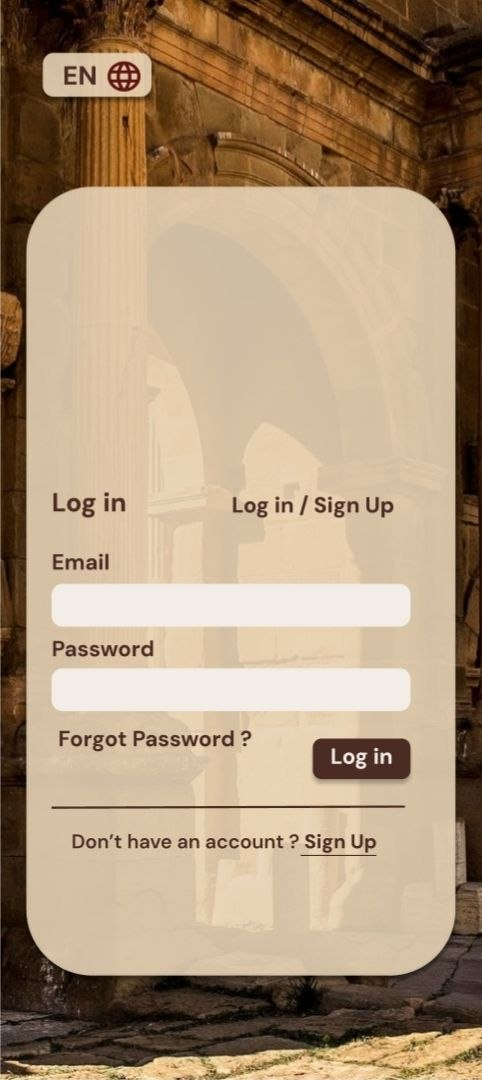
\includegraphics[width=0.8\linewidth]{images/log in.jpg}
\end{minipage}
\begin{minipage}{0.33\textwidth}
\centering
    \textbf{Sign Up page}
    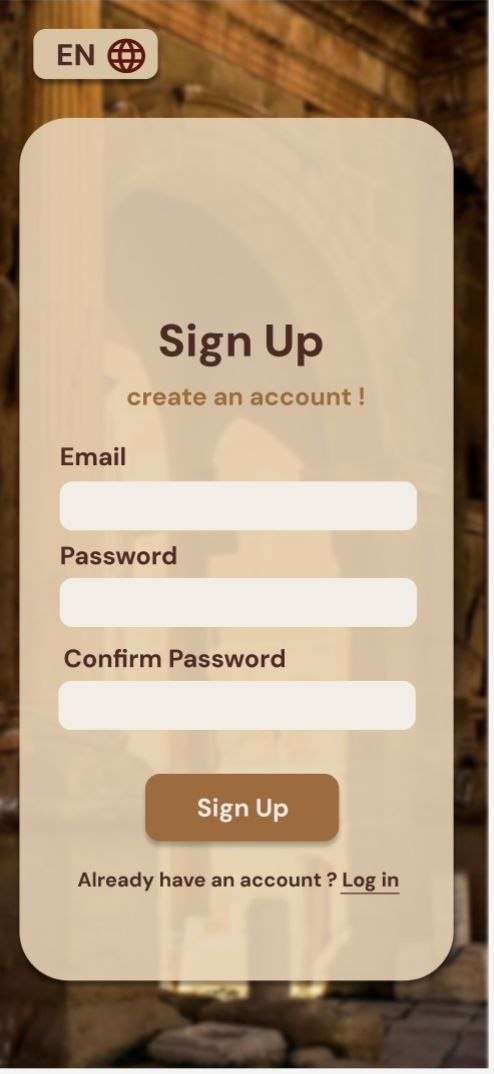
\includegraphics[width=0.8\linewidth]{images/sign up.jpg} 
\end{minipage}
\begin{minipage}{0.33\textwidth}
\centering
    \textbf{Forget password page}
    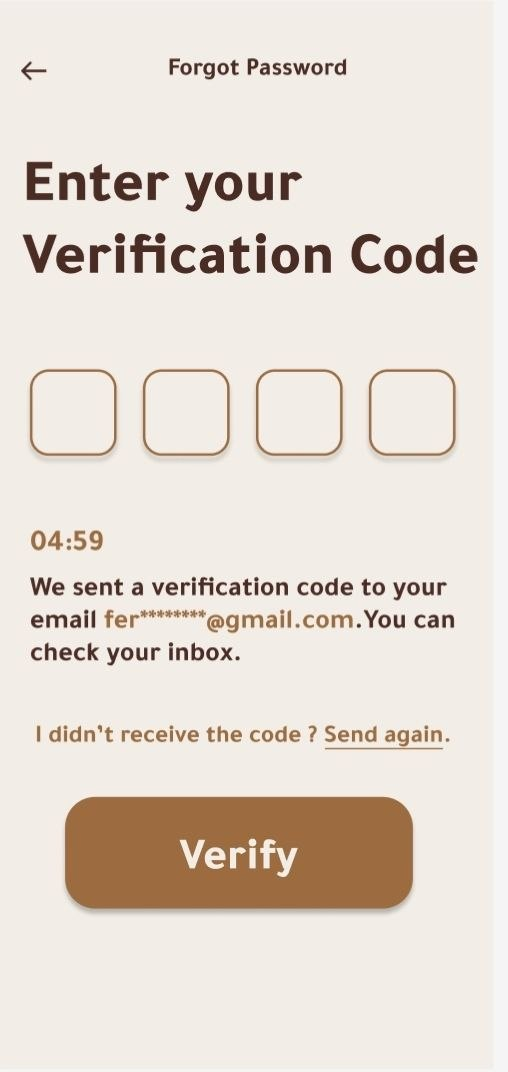
\includegraphics[width=0.8\linewidth]{images/forget password.jpg}
\end{minipage}
\begin{minipage}{0.33\textwidth}
\centering
   \textbf{Home page}
   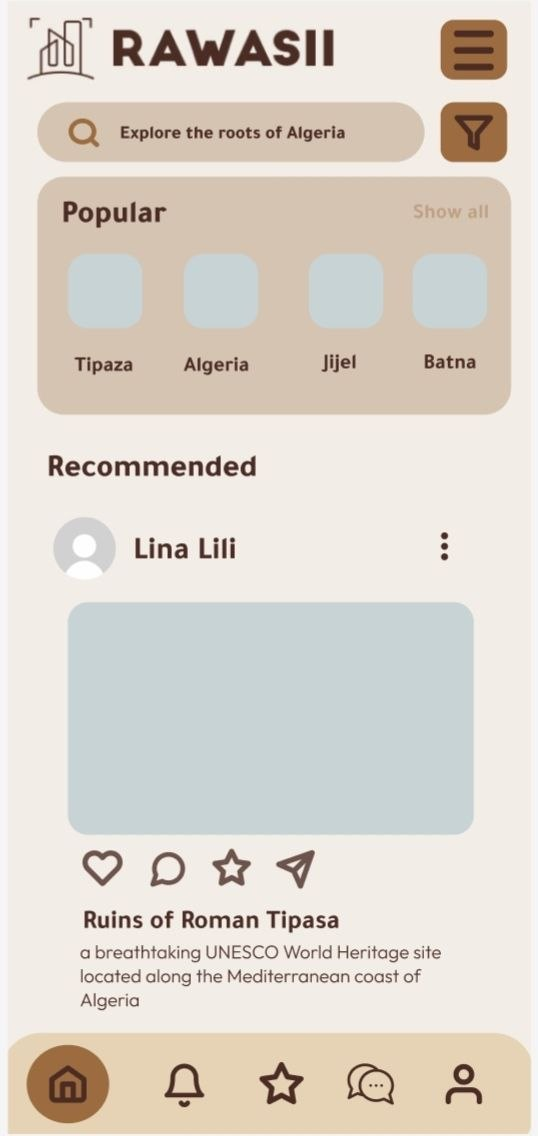
\includegraphics[width=0.8\linewidth]{images/home page.jpg}
\end{minipage}
\begin{minipage}{0.33\textwidth}
\centering
    \textbf{Profile page}
    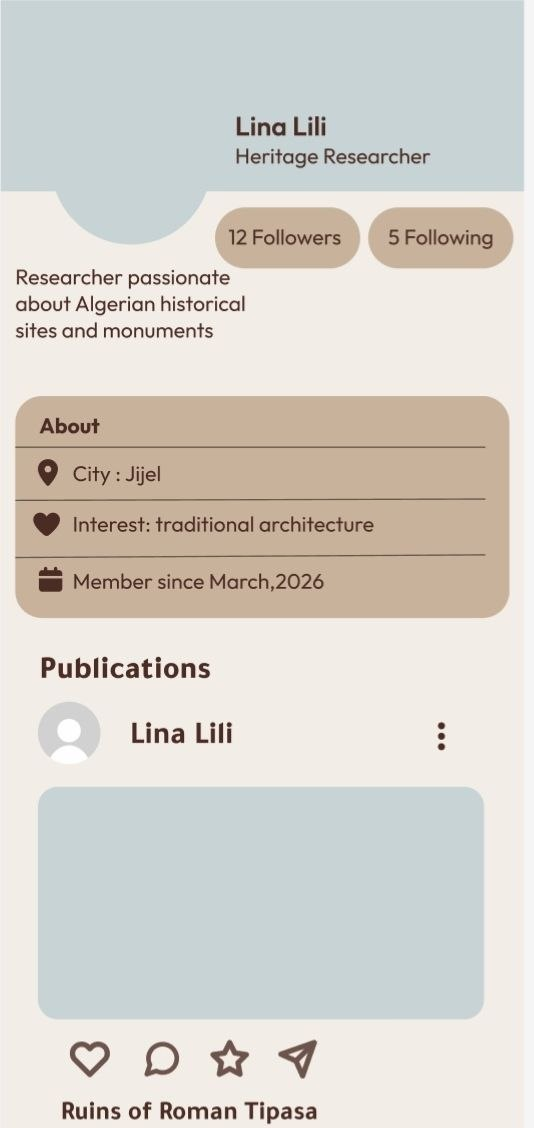
\includegraphics[width=0.8\linewidth]{images/profile page 2.jpg} 
\end{minipage}
\begin{minipage}{0.33\textwidth}
\centering
    \textbf{Notifications page}
    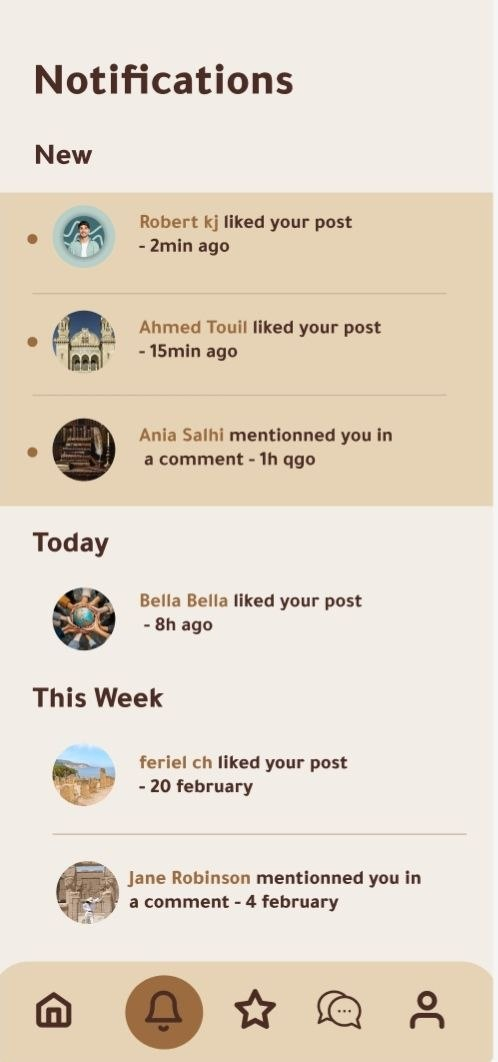
\includegraphics[width=0.8\linewidth]{images/notifications.jpg}
\end{minipage}
\begin{minipage}{0.33\textwidth}
\centering
   \textbf{Admin panel page}
   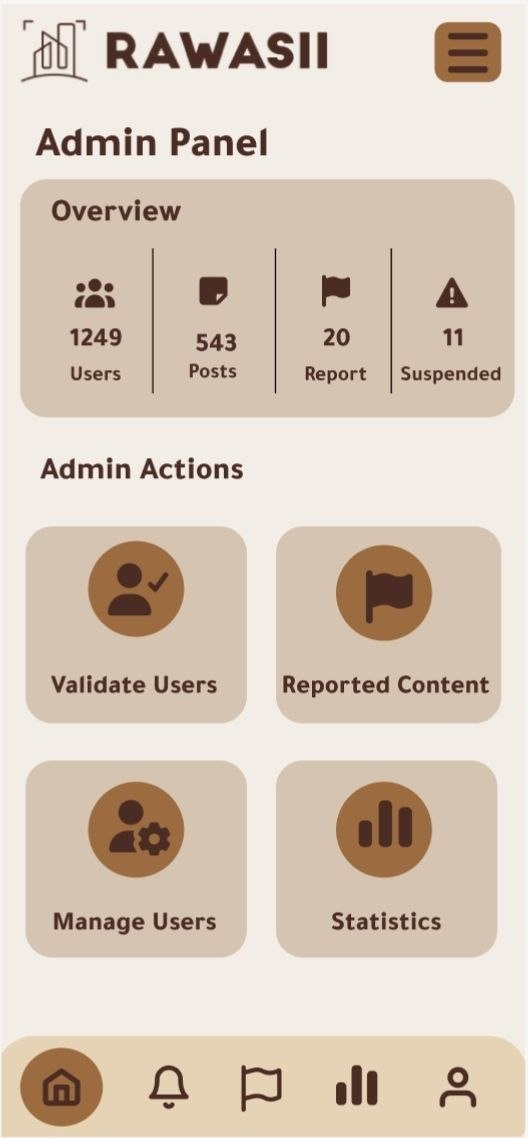
\includegraphics[width=0.8\linewidth]{images/admin panel.jpg}
\end{minipage}
\begin{minipage}{0.33\textwidth}
\centering
    \textbf{Add post}
    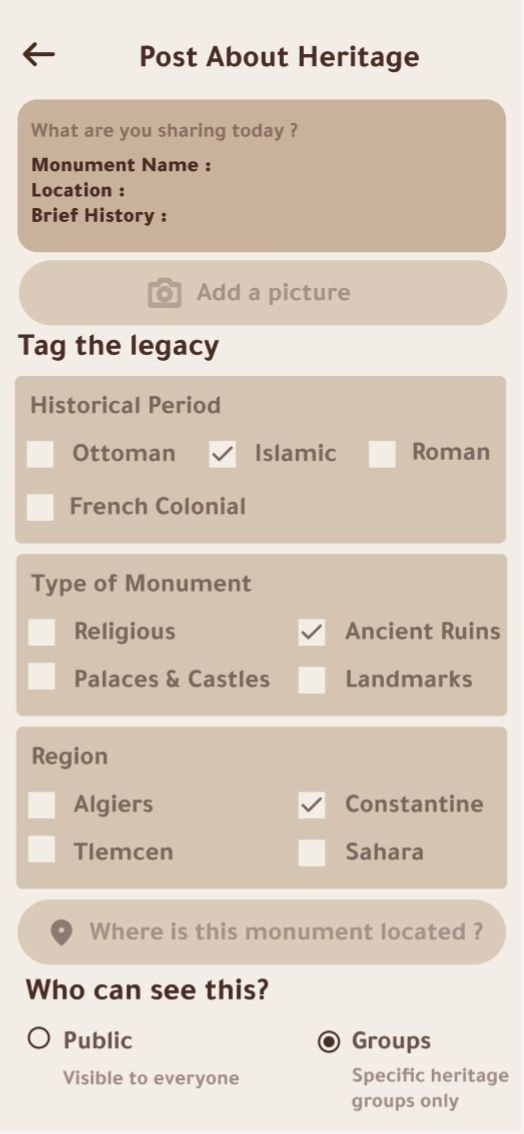
\includegraphics[width=0.8\linewidth]{images/add post.jpg}  
\end{minipage}
\begin{minipage}{0.33\textwidth}
\centering
    \textbf{Edit profile}
    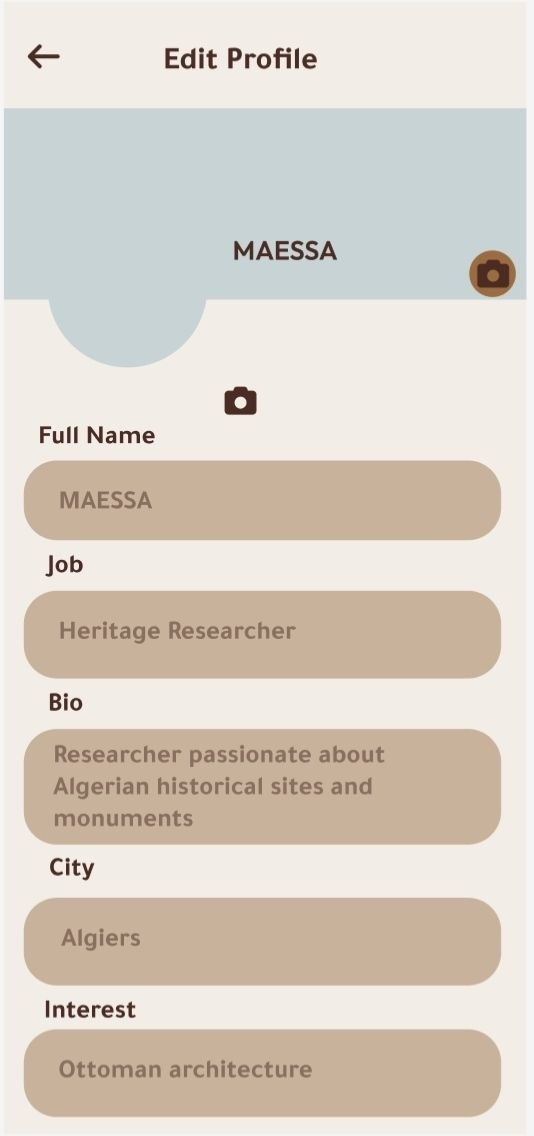
\includegraphics[width=0.8\linewidth]{images/edit profile.jpg}
\end{minipage}
\begin{minipage}{0.33\textwidth}
\centering
   \textbf{Comments}
   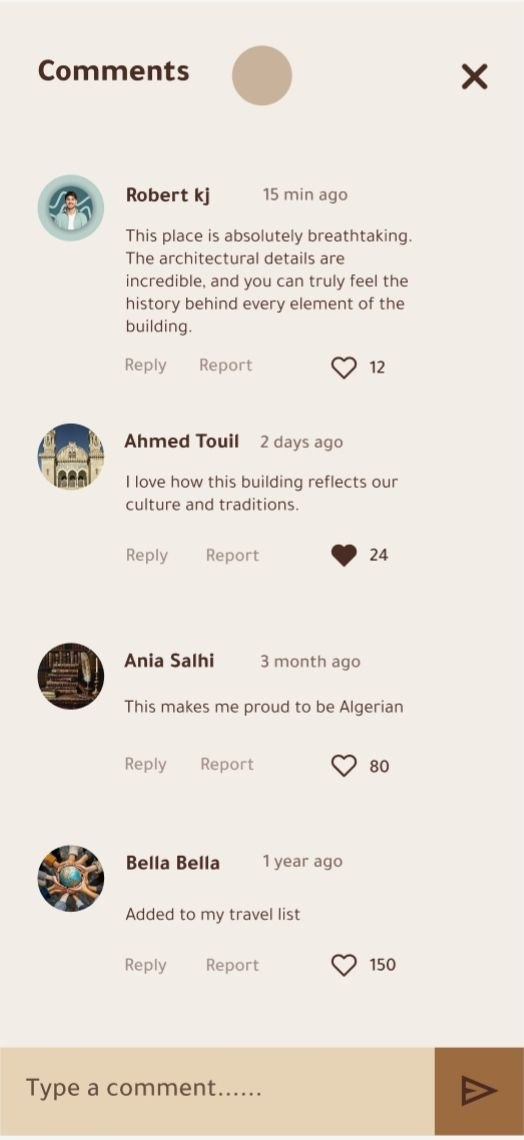
\includegraphics[width=0.8\linewidth]{images/comments.jpg}
\end{minipage}
\begin{minipage}{0.33\textwidth}
\centering
    \textbf{Statistics}
    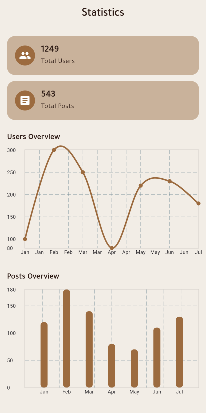
\includegraphics[width=0.8\linewidth]{images/statust.png}  
\end{minipage}
\begin{minipage}{0.33\textwidth}
\centering
    \textbf{visits page}
    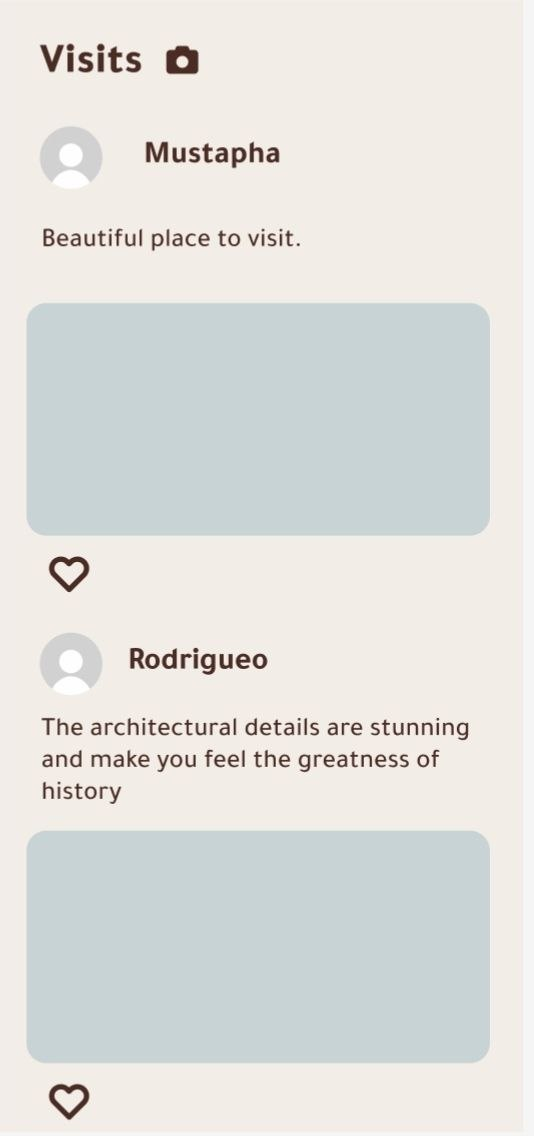
\includegraphics[width=0.8\linewidth]{images/visits.jpg}
\end{minipage}
\begin{minipage}{0.33\textwidth}
\centering
   \textbf{Validate users}
   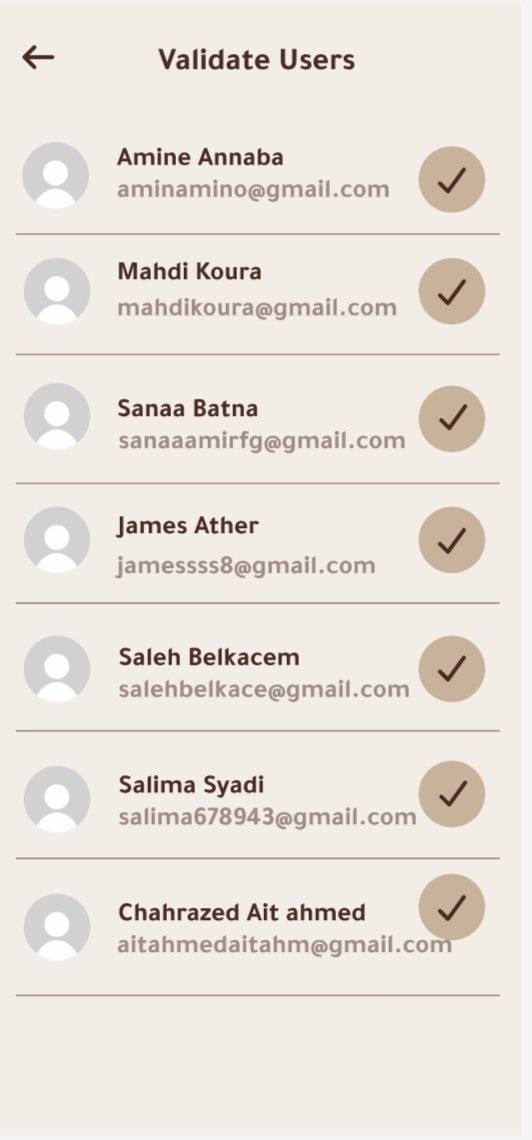
\includegraphics[width=0.8\linewidth]{images/validate users.jpg}
\end{minipage}
\begin{minipage}{0.33\textwidth}
\centering
    \textbf{Explore}
    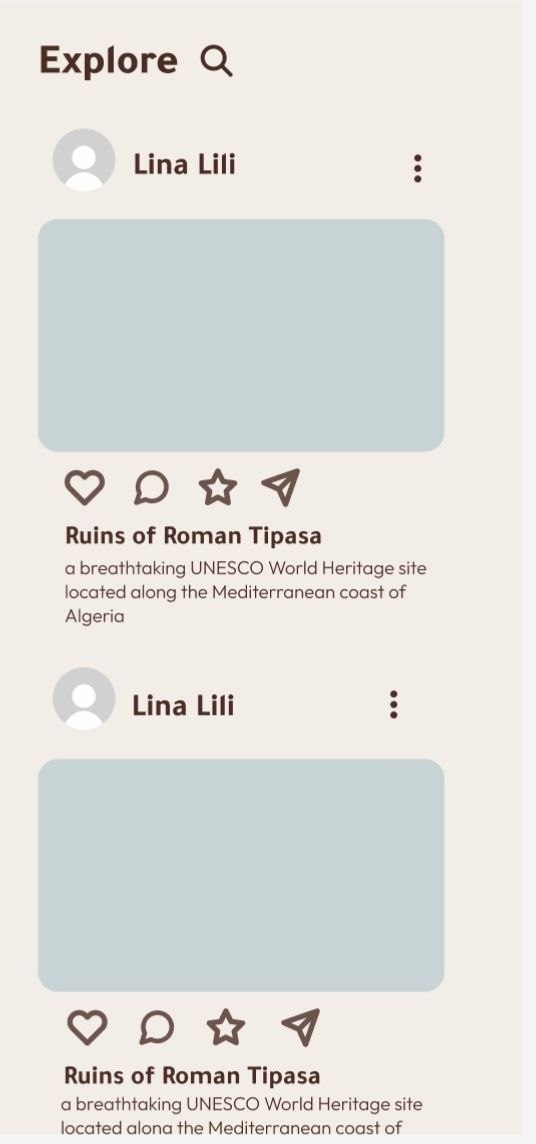
\includegraphics[width=0.8\linewidth]{images/explore.jpg}  
\end{minipage}
\begin{minipage}{0.33\textwidth}
\centering
    \textbf{Manage users }
    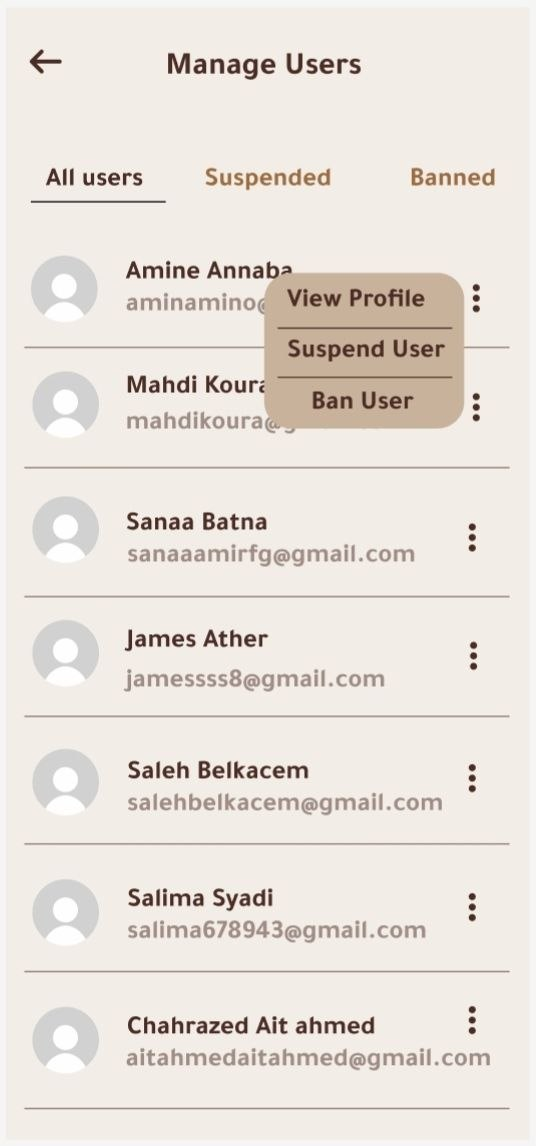
\includegraphics[width=0.8\linewidth]{images/manage users.jpg} 
\end{minipage}

\subsection{Back-end}
\subsubsection{Introduction}
The backend is a core component of the application responsible for handling business logic, managing data, and enabling communication between the frontend and the database. It acts as an intermediary layer that receives user requests, processes them, and returns appropriate responses in a structured and secure way.

The backend was developed using the Dart programming language with the help of the Dart Frog framework, which provides a modern and lightweight environment for building RESTful APIs and server-side applications. In addition, Supabase was used to manage the database and authentication services in a cloud-based environment.
\subsubsection{Application Logic Using Dart and Dart Frog}
The Dart language was used to implement the application’s core logic, including data processing, input validation, and controlling the flow of operations within the system. This
allowed the creation of a clean and well-organized codebase that is easy to maintain and
modify.

In addition, Dart Frog was used to build the backend of the application. This framework provides a modern way to create APIs using Dart, allowing the development of lightweight and fast REST-based servers. It also helped structure the project by separating responsibilities, making the code more readable and easier to maintain.
\subsubsection{Code Structure and Architecture}
\begin{minipage}{0.7\textwidth}
The code was organized in a modular and structured way to improve readability, maintainability, and scalability. The project was divided into separate files and layers, where each part is responsible for a specific functionality such as request handling, database communication, and business logic.

This separation of concerns helped reduce code complexity and made it easier to maintain and extend the application in the future. Each module is independent, which allows developers to modify or add features without affecting other parts of the system.
\end{minipage}
\begin{minipage}{0.3\textwidth}
\centering
    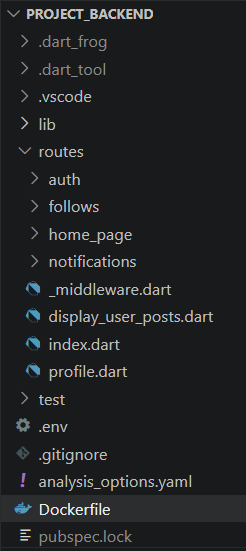
\includegraphics[width=0.8\linewidth]{images/backend.png}
\end{minipage}

\subsubsection{API Development (Endpoints)}
The backend APIs were developed using Dart Frog to handle communication between the application and the backend system. These APIs act as endpoints that receive HTTP requests from the frontend, process the data, and return appropriate responses.

A set of RESTful endpoints was created to support the main operations of the application, including retrieving data, adding new records, updating existing data, and deleting records.

Although Supabase provides built-in auto-generated APIs for database operations, custom endpoints were also implemented using Dart Frog to handle application-specific business logic and ensure better control over data processing.
\subsubsection{Database Integration}
Supabase was used as a cloud-based backend solution for database management. The application is directly connected to the Supabase database, enabling real-time operations such as inserting, retrieving, updating, and deleting data.

Supabase is built on PostgreSQL and provides an integrated environment that simplifies backend development by offering authentication, database management, and API services in one platform. The data is organized into relational tables to ensure consistency, reduce redundancy, and improve performance.
\subsubsection{Data Flow in the Application}
Requests are sent from the frontend to the Dart Frog backend, where they are received,
processed, and validated. The backend then communicates with Supabase to retrieve or
update data, and finally sends the response back to the application for display.

This flow ensures a well-structured system where data handling is organized, secure, and
efficient.
\subsubsection{Authentication and Authorization}
User authentication was implemented using Supabase authentication services to securely manage user login and account creation. This ensures that only verified users can access the application.
In addition to authentication, an authorization system was applied to control user permissions and define what actions each user is allowed to perform. This helps protect sensitive data and ensures proper access control within the application.
\subsubsection{Testing the Backend APIs}
\begin{minipage}{0.4\textwidth}
   To ensure the proper functioning of the backend, the APIs were tested using Thunder Client. This tool was used to send requests to different endpoints and verify that the backend built with Dart Frog is working correctly and is able to communicate with Supabase.

The testing process focused on checking the structure of the requests and ensuring that the endpoints respond as expected. Although only the request configuration is documented in the report, the tests confirmed that the API operations (such as data retrieval and submission) were successfully executed during development.
\end{minipage}
\begin{minipage}{0.6\textwidth}
\centering
    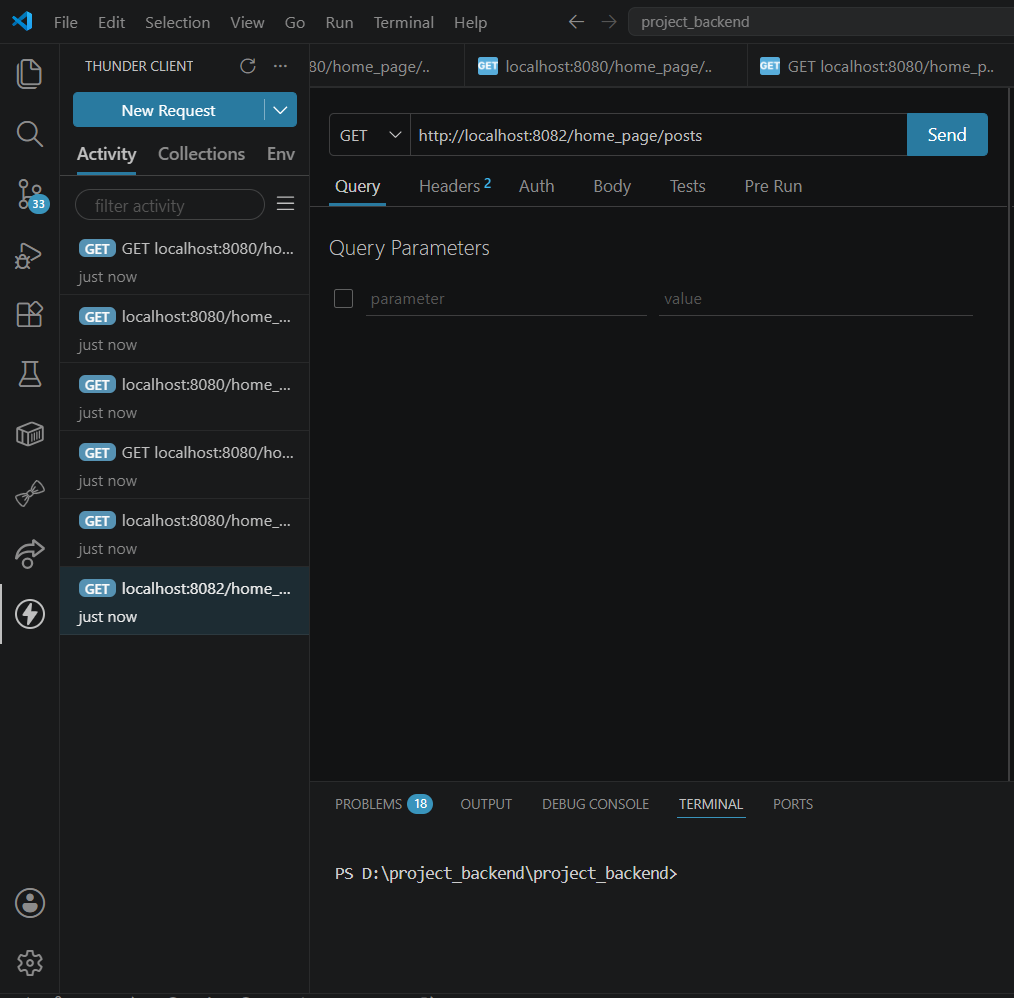
\includegraphics[width=0.9\linewidth]{images/Thunder client.png}
\end{minipage}
\subsubsection{Conclusion}
The backend system was successfully developed using Dart and the Dart Frog framework, combined with Supabase for database and authentication management. This combination resulted in a fast, scalable, and well-structured backend architecture.

The clear code organization, well-designed APIs, and secure authentication system contributed to building a reliable and efficient application capable of handling data operations effectively while ensuring maintainability and future scalability.


\begin{minipage}{0.5\textwidth}
\centering
    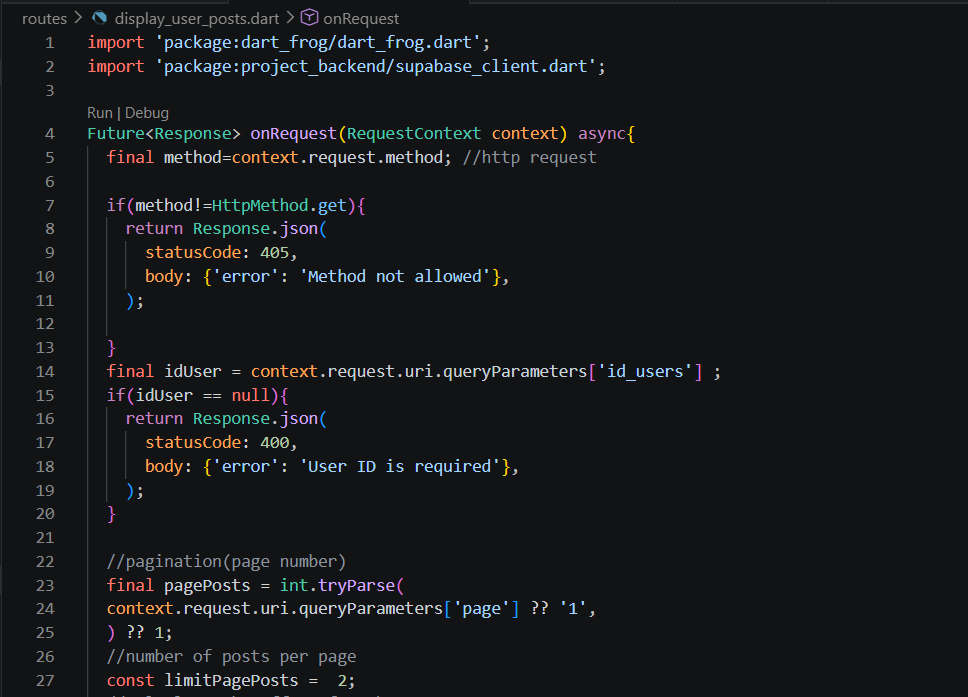
\includegraphics[width=1\linewidth]{images/back1.png}
\end{minipage}
\begin{minipage}{0.5\textwidth}
\centering
    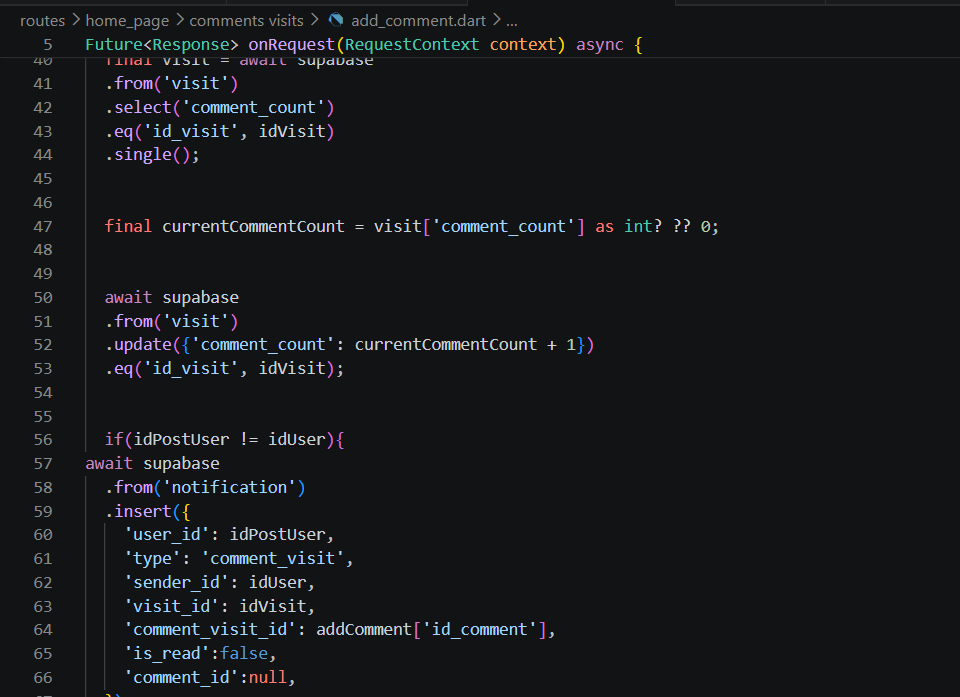
\includegraphics[width=1\linewidth]{images/back2.png}
\end{minipage}


\subsection{Integration}
\subsubsection{Introduction}
The integration phase focuses on connecting all parts of the application to ensure that the system works as a single unified product. This stage involves linking the frontend, backend, and database to enable smooth and accurate data exchange between all components.
\subsubsection{Frontend and Backend Integration}
The frontend was connected to the backend developed using Dart Frog through RESTful APIs. This integration allows the user interface to send requests to the server, where they are processed and appropriate responses are returned and displayed in the application.

This connection makes the application dynamic, as the displayed data changes based on user interactions in real time.
\subsubsection{Backend and Database Integration}
The backend was integrated with Supabase for cloud-based data management. Through this integration, core operations such as inserting, retrieving, updating, and deleting data were efficiently performed in an organized manner.

Supabase provided a ready-to-use database environment, which simplified communication between the backend and stored data while ensuring consistency and reliability.
\subsubsection{Authentication Integration}
The Supabase authentication system was integrated into the application to securely manage user registration and login. This integration ensures that only authenticated users can access specific features of the system, helping protect data and manage user permissions effectively.
\subsubsection{Data Flow in the System}
Data is exchanged through APIs built with Dart Frog. Requests are sent from the frontend to the backend, processed accordingly, and then the backend communicates with the database when needed. Finally, the response is returned to the frontend to be displayed to the user.
\subsubsection{Conclusion}
The integration phase successfully connected all components of the application into a unified system. The use of Dart Frog and Supabase ensured smooth communication between layers, improved data organization, and provided a stable and efficient user experience.
\subsection{Deployment and Hosting}
To deploy and host the backend system, Railway was used as the cloud hosting platform. Railway provides a simple deployment environment and offers free resources for testing purposes, including temporary storage and runtime usage that were sufficient for hosting and testing the project during development.

In order to deploy the application successfully, the backend source code was uploaded to GitHub, allowing Railway to access and deploy the project directly from the repository.

The deployment process also required the use of Docker. Docker was used to containerize the application and define the execution environment needed for the backend to run correctly on the hosting platform. Additional configuration files were created to manage dependencies, runtime settings, and deployment instructions required by Railway.

This deployment setup helped ensure that the backend could run consistently and be accessible online while simplifying the hosting and environment configuration process.

\begin{center}
    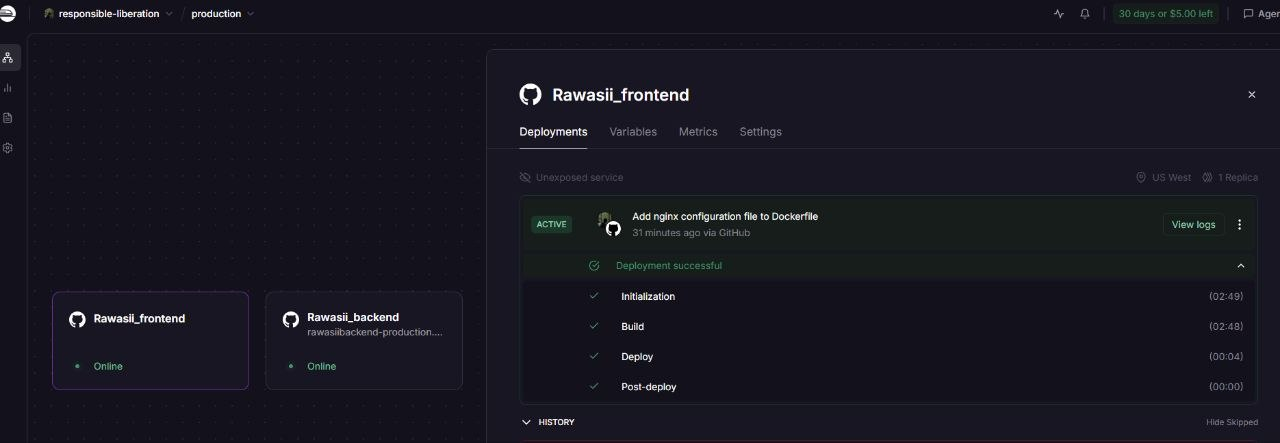
\includegraphics[width=1\linewidth]{images/hosting.jpg}
\end{center}

\newpage

\section{Conclusion}

Our project centered around the design and development of a social platform dedicated to the promotion of Algerian architectural heritage, addressing a concrete problem: the absence of a unifying digital space allowing heritage enthusiasts to share knowledge, interact, and mobilize around a common cause.

We began with an in-depth analysis of the project specifications and existing similar applications, in order to identify the essential features to be integrated and the gaps to be filled. This phase was followed by a detailed design of the system architecture, accompanied by rigorous task planning and proactive risk anticipation.

Development was organized around a decoupled architecture: a RESTful backend built with Dart Frog and Supabase, handling user management, publications, social interactions and notifications, and a mobile frontend developed with Flutter. The application was containerized using Docker to facilitate deployment and system portability.

Throughout the project, continuous testing was carried out to ensure the reliability of the implemented features, and comprehensive technical documentation was produced to support both users and developers in working with the platform.

\subsection{Skills Acquired}
\begin{itemize}
    \item Backend architecture: We gained practical mastery of RESTful API development, relational database management with Supabase, and the implementation of authentication and data security mechanisms.
    \item Mobile development: Building the frontend with Flutter allowed us to understand the specific challenges of developing modern, responsive, and user-friendly mobile interfaces.
    \item  Project management: Coordinating between team members, meeting deadlines, and adapting to unexpected constraints strengthened our collaborative project management skills.
    \item DevOps and deployment: Setting up a Docker environment and exploring cloud deployment solutions introduced us to the real-world challenges of deploying a web application to production.
    \item Self-directed learning: Faced with technologies not covered in our curriculum, we developed the ability to learn independently from official documentation, thereby reinforcing our technical autonomy.
\end{itemize}
\subsection{Perspectives}
On the functional side, several improvement areas were identified but could not be integrated within the current scope of the project:
\begin{itemize}
    \item Production deployment: The stable deployment of the application on a cloud infrastructure remains a short-term priority, requiring adaptation of the build environment to the Dart Frog framework.
    \item Personalized news feed: Implementing a recommendation algorithm based on each user's preferences and subscriptions would considerably enrich the browsing experience.
    \item Advanced moderation features: Developing more complete administrative tools, including detailed statistics and an automated reporting system, would strengthen community governance.

\vspace{0.5cm}

In the long term, the platform could evolve into a fully integrated digital ecosystem dedicated to Algerian heritage, incorporating advanced geolocation features, interactive mapping, and collaboration between cultural institutions, thereby contributing to the preservation and promotion of the national architectural heritage.
\end{itemize}


\end{document}
